%% Elsevier elsarticle manuscript for:
%% Progress in Biophysics and Molecular Biology
%% Special Issue: Biophysics and Molecular Biology for Space Flight (SI 337891)
\documentclass[final,5p,times,twocolumn,numbers,sort&compress]{elsarticle}

\usepackage[utf8]{inputenc}
\usepackage[T1]{fontenc}
% geometry handled by 5p elsarticle
\usepackage{graphicx}
\usepackage{amsmath,amssymb,amsfonts}
\usepackage{booktabs}
\usepackage{longtable}
\usepackage{multirow}
\usepackage{array}
\usepackage{xcolor}
\usepackage{url}
\usepackage{xr}
\usepackage[colorlinks=true,linkcolor=blue!55!black,citecolor=blue!55!black,urlcolor=blue!55!black]{hyperref}

\externaldocument{supplementary}
\graphicspath{{figures/}}

\journal{Progress in Biophysics and Molecular Biology (Special Issue: Biophysics and Molecular Biology for Space Flight)}

% Unit and formula helpers
\newcommand{\ums}{\ensuremath{\mu\mathrm{mol\,m^{-2}\,s^{-1}}}}
\newcommand{\umh}{\ensuremath{\mu\mathrm{mol\,h^{-1}\,cm^{-2}}}}
\newcommand{\cmsu}{\ensuremath{\mathrm{cm\,s^{-1}}}}
\newcommand{\mseu}{\ensuremath{\mathrm{m^{2}\,s^{-1}}}}
\newcommand{\molms}{\ensuremath{\mathrm{mol\,m^{-2}\,s^{-1}}}}
\newcommand{\msq}{\ensuremath{\mathrm{m\,s^{-2}}}}
\newcommand{\co}{CO\textsubscript{2}}
\newcommand{\oo}{O\textsubscript{2}}
\newcommand{\wo}{H\textsubscript{2}O}

\begin{document}
\sloppy

\begin{frontmatter}

\title{From microgravity boundary-layer biophysics to the spaceflight multi-ome: a coupled lattice-Boltzmann and Farquhar--von Caemmerer--Berry model of \textit{Arabidopsis} gas exchange and enclosure carbon starvation}

\author[purdue]{Richard J. Barker\corref{cor1}}
\ead{dr.richard.barker@gmail.com}
\cortext[cor1]{Corresponding author. ORCID: 0000-0001-5681-9857.}

\affiliation[purdue]{organization={Purdue University},
            city={West Lafayette},
            state={IN},
            country={USA}}

\begin{highlights}
\item Removing gravity eliminates buoyant plumes and cuts leaf $g_{bl}$ by $2.0\text{--}2.3\times$.
\item Forced ventilation reverses the microgravity penalty ($2.0\,\mathrm{cm\,s^{-1}}$ leaf, $6.1$ rosette).
\item Lit sealed canisters exhaust headspace $\mathrm{CO_2}$ in $\sim 7\,\mathrm{min}$ ($1\%$ 12-h carbon gain).
\item Canister $\mathrm{CO_2}$ starvation dominates the $1\,g$ vs $\mu g$ boundary-layer gap by $22\times$.
\item OSDR omics confirms carbon starvation; illumination separates all 6 contrasts ($p=0.05$).
\end{highlights}

\begin{graphicalabstract}
\centering
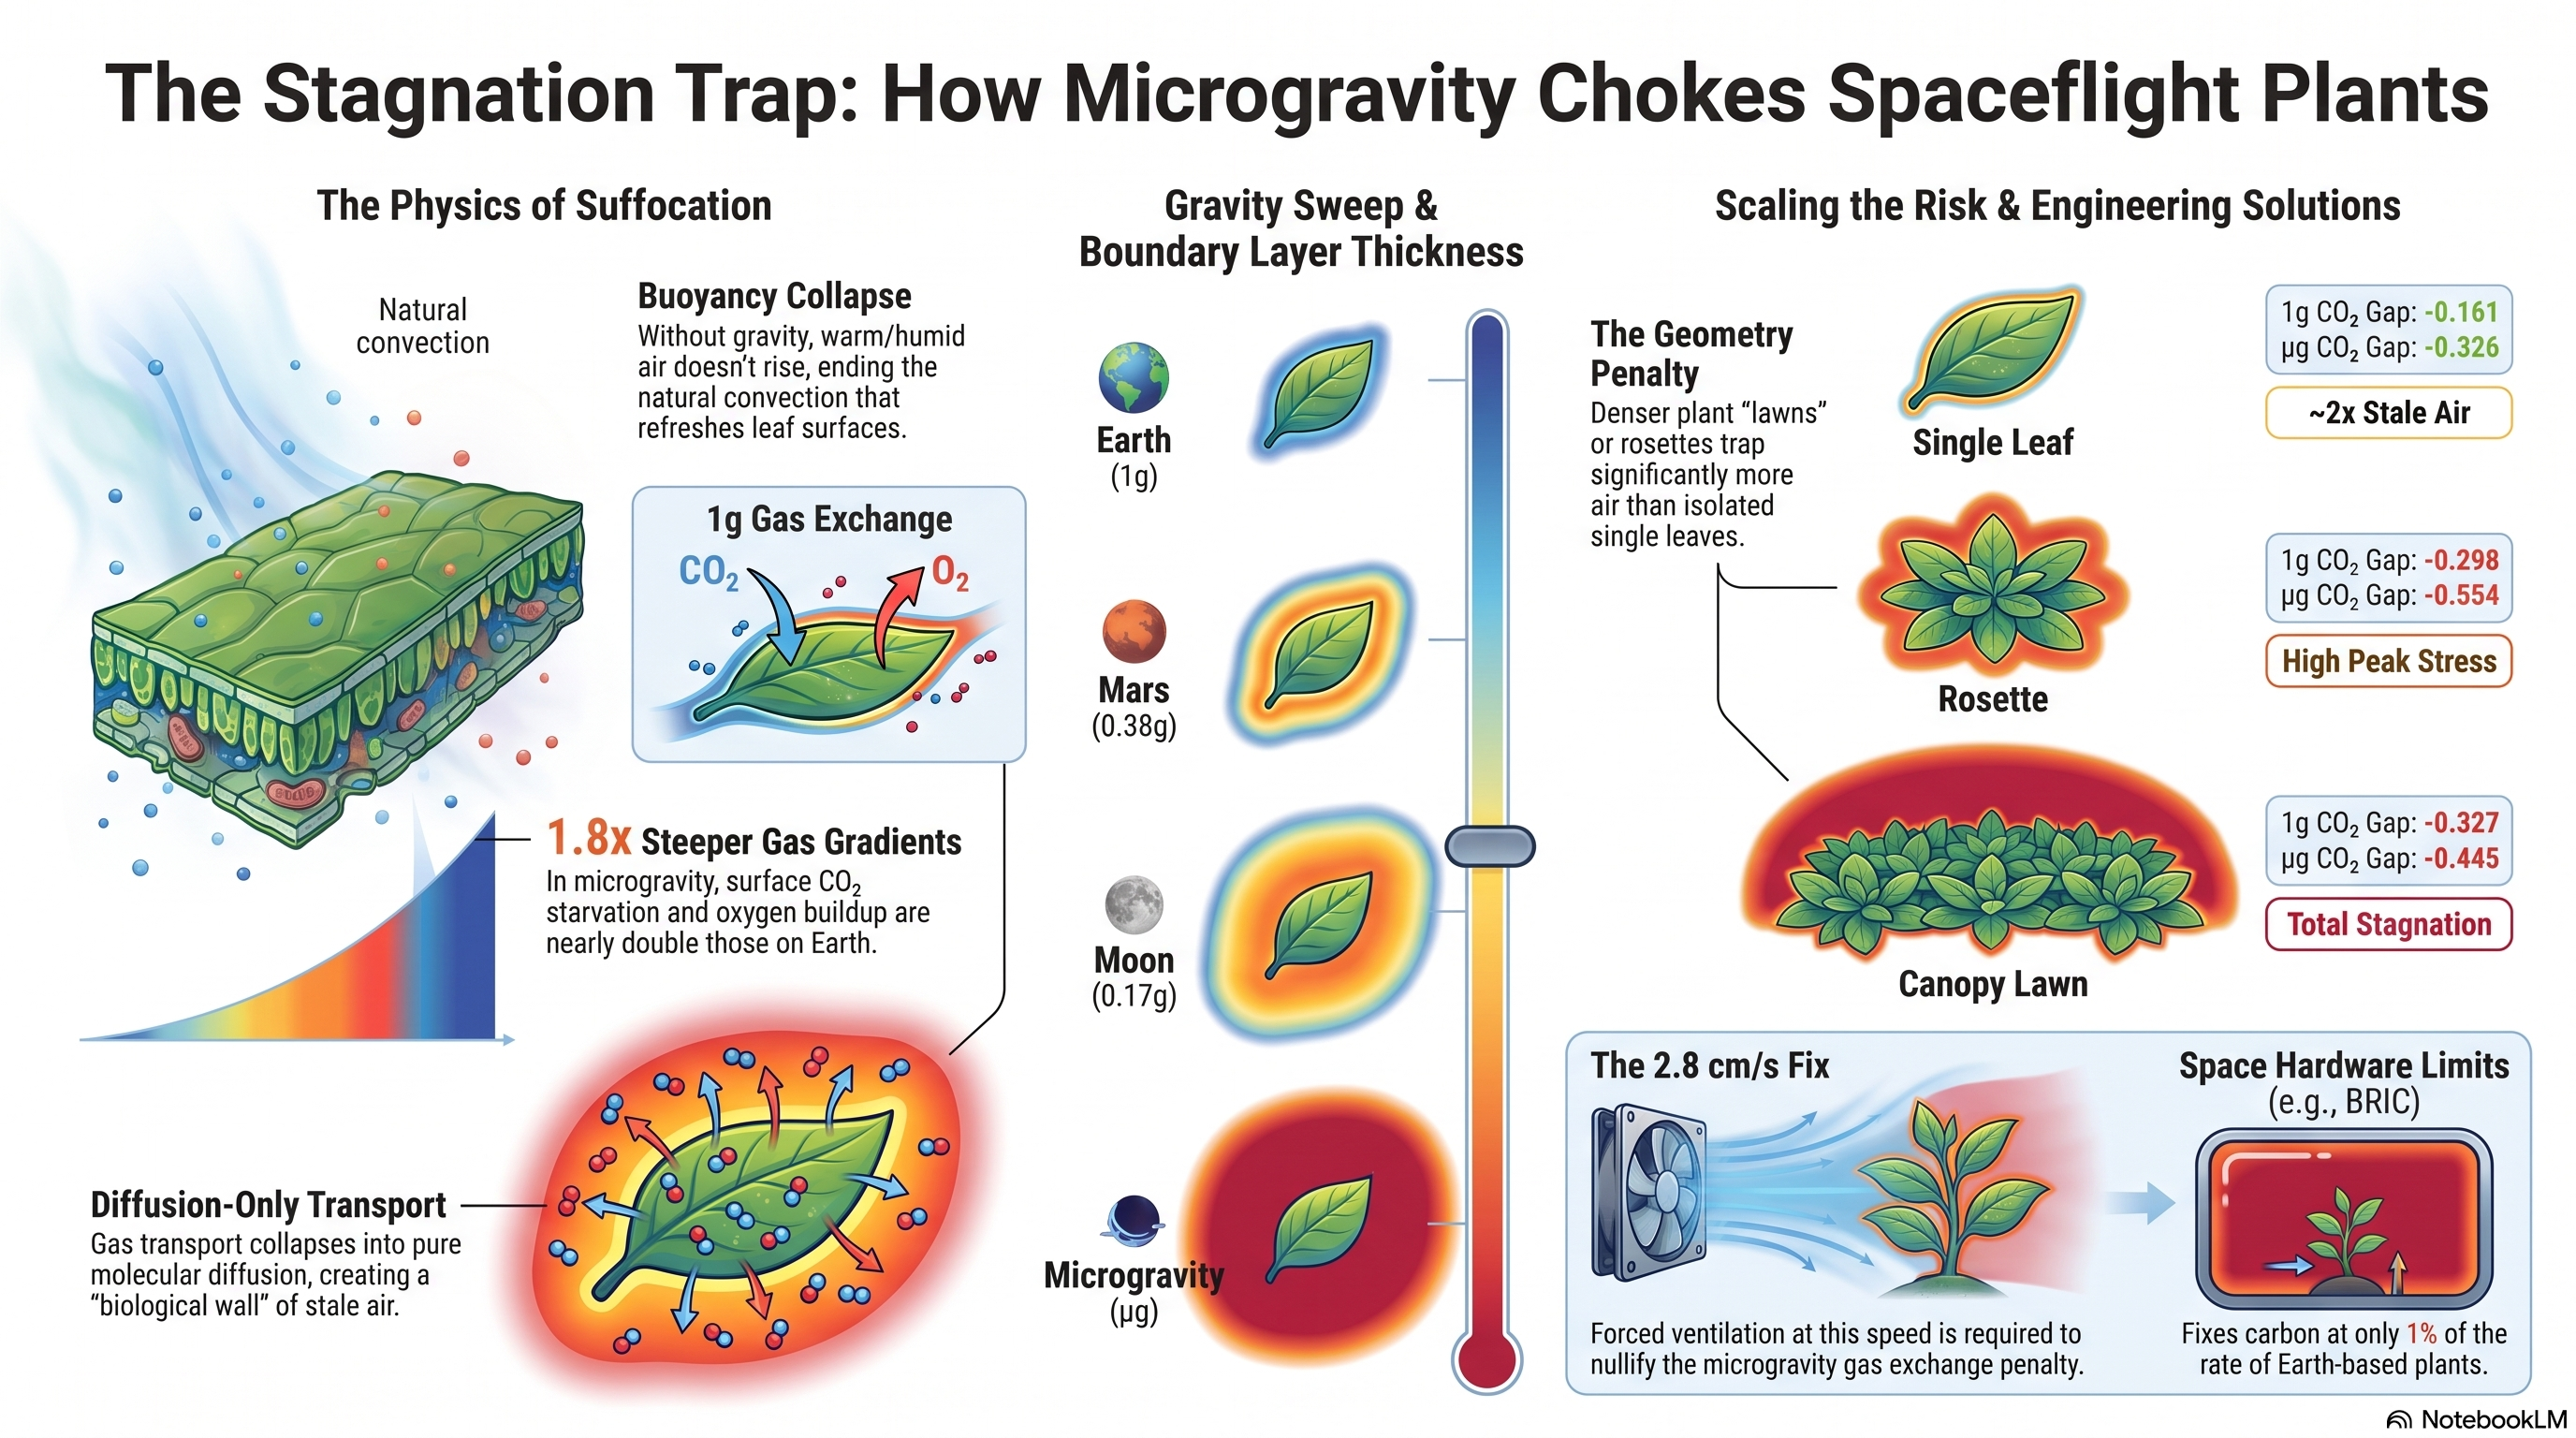
\includegraphics[width=0.95\textwidth]{Microgravity_Stagnation_in_Spaceflight_Plants.png}
\end{graphicalabstract}

\begin{abstract}
Plants grown in spaceflight display conserved transcriptional and proteomic stress signatures whose physical origin remains debated. Two distinct gas-transport mechanisms have been proposed: the microgravity loss of buoyancy-driven free convection, which thickens the unstirred diffusive boundary layer around leaves, and atmospheric stagnation inside sealed or poorly ventilated spaceflight growth hardware. Because no flight experiment has resolved sub-millimetre leaf boundary layers or logged in-canister $\mathrm{CO_2}$ across hardware classes, we built an end-to-end biophysical and multi-omics framework to test both mechanisms quantitatively. First, we implemented a two-dimensional D2Q9/D2Q5 lattice-Boltzmann computational fluid dynamics (CFD) solver for incompressible flow, multi-species ($\mathrm{CO_2}$, $\mathrm{O_2}$, $\mathrm{H_2O}$) advection--diffusion, and solutal Boussinesq buoyancy under an adjustable gravity vector ($1\,g \to \text{Mars } 0.38\,g \to \text{Moon } 0.17\,g \to \mu g$), validated against four numerical benchmarks (lid-driven cavity, K\'arm\'an cylinder wake, natural-convection cavity to $0.18\%$ on Nusselt number, and analytic $\mathrm{erfc}$ diffusion) and anchored to empirical \textit{Arabidopsis thaliana} whole-chamber gas exchange ($A = 3.85\,\ums$). Removing gravity eliminates convective plumes ($u_{\max}\propto\sqrt{g}\to 0$), reducing leaf boundary-layer conductance $g_{bl}$ from $0.997$ to $0.443\,\molms$ for an isolated leaf, $0.540$ to $0.272\,\molms$ for a rosette, and $0.133$ to $0.058\,\molms$ for a dense microgreen canopy. Forced ventilation reverses this microgravity penalty, but the Earth-equivalent airflow scales with planting density from $\approx 2.0\,\cmsu$ (leaf) to $\approx 6.1\,\cmsu$ (rosette). Second, we coupled the CFD-derived $g_{bl}$ values and zero-dimensional (0-D) hardware mass balances for three International Space Station growth systems---sealed Biological Research in Canisters (BRIC), micropore-taped Characterizing Arabidopsis Root Attractions (CARA), and actively ventilated Vegetable Production System (VEGGIE)---to a Farquhar--von Caemmerer--Berry (FvCB) $\mathrm{C_3}$ model with explicit Rubisco oxygenation ($\varphi = V_o/(V_o+V_c)$). An illuminated sealed BRIC canister draws its headspace $\mathrm{CO_2}$ down to the compensation point within $\sim 7\,\mathrm{min}$, collapsing 12\,h carbon gain to $\approx 1\%$ of an unenclosed control (versus $\approx 90\%$ for CARA and $\approx 100\%$ for VEGGIE) and raising $\varphi$ from $18.0\%$ to $46.2\%$ at experimental irradiance ($60\,\ums$). Because canister drawdown is a mass balance, it occurs symmetrically in both flight and ground controls: it cancels out of the published flight-versus-ground contrast while shifting the baseline metabolic state into severe carbon starvation (an enclosure effect $\approx 22\times$ larger than the microgravity boundary-layer effect). Furthermore, contrary to our starting hypothesis, $\mathrm{CO_2}$ exhaustion causes the $1\,g$ and $\mu g$ boundary layers to converge rather than diverge as photosynthetic flux vanishes, leaving a residual microgravity assimilation deficit of $<3\%$ at leaf/rosette scale and up to $11\%$ in a dense canopy at $60\,\ums$ ($5\text{--}9\%$ and $26\text{--}29\%$ at saturating light). Third, after an exhaustive census of all 567 studies in the NASA Open Science Data Repository (OSDR) revealed zero plant metabolomics datasets (0 of 12 metabolomics studies), we formulated a falsifiable 21-compound flux-propagated metabolite scaffold and tested the coupled model against OSD-522 (BRIC-LED) shoot transcriptomics and proteomics and across six matched flight-versus-ground contrasts from five OSDR studies. In OSD-522, the model called eight of nine transcriptome gene-set responses and four of seven in the proteome (repression of photosystems, Rubisco, carbon fixation, and starch/sucrose metabolism; induction of \textit{DIN6/ASN1} carbon-starvation markers; maintenance of photorespiratory enzymes above Rubisco). Multi-omics pathway integration in PaintOmics 4 showed that endoplasmic reticulum protein processing (unfolded protein response, $p = 8.6\times 10^{-9}$) dominates the global response while photorespiration ranks in the bottom $8\%$ (214th of 232 pathways). Across the six OSDR contrasts, illumination separated every lit study from every dark study on carbon starvation over photosynthesis ($p = 0.05$), whereas enclosure class alone did not. We conclude that unlogged enclosure atmosphere is a first-order covariate in spaceflight plant biology and outline the in-canister sensor logging, 20-compound targeted metabolomics panel, and three-arm / $2\times 2$ factorial experimental designs required to separate hardware carbon starvation from microgravity.
\end{abstract}

\begin{keyword}
microgravity \sep boundary layer \sep computational fluid dynamics \sep lattice-Boltzmann \sep Farquhar--von Caemmerer--Berry \sep photorespiration \sep \textit{Arabidopsis thaliana} \sep spaceflight growth hardware \sep multi-omics \sep NASA OSDR
\end{keyword}

\end{frontmatter}

%=============================================================================
\section{Introduction}\label{sec:intro}
%=============================================================================

On Earth, a photosynthesising or transpiring leaf warms and humidifies the thin layer of air in contact with its epidermis. Because water vapour ($M = 18\,\mathrm{g\,mol^{-1}}$) is lighter than dry air ($M \approx 29\,\mathrm{g\,mol^{-1}}$), the humidified boundary layer is buoyant and rises in a free-convection plume that continuously sweeps the leaf surface, replenishing $\mathrm{CO_2}$ while removing $\mathrm{O_2}$ and water vapour. This buoyancy-driven ventilation is invisible under terrestrial conditions, yet it sets the still-air boundary-layer conductance ($g_{bl}$) that acts in series with stomatal ($g_s$) and mesophyll ($g_m$) conductances to govern the chloroplastic $\mathrm{CO_2}$ mole fraction ($C_c$) reaching Rubisco:
\begin{equation}
C_a \xrightarrow{\;g_{bl}\;} C_s \xrightarrow{\;g_s\;} C_i \xrightarrow{\;g_m\;} C_c ,
\label{eq:conductance_chain}
\end{equation}
where $C_a$, $C_s$, and $C_i$ denote the bulk enclosure, leaf-surface, and intercellular $\mathrm{CO_2}$ mole fractions, respectively.

In microgravity ($\mu g$), hydrostatic pressure gradients and buoyancy-driven natural convection vanish. In the absence of forced ventilation, gas transport outside the organ collapses to pure molecular diffusion, thickening the unstirred boundary layer ($\delta$) and steepening the surface-to-bulk concentration gaps ($\Delta C$) of $\mathrm{CO_2}$, $\mathrm{O_2}$, and $\mathrm{H_2O}$ \citep{porterfield2002,kitaya2003}. For decades, this boundary-layer thickening has been invoked to explain the hypoxia, oxidative stress, altered carbon metabolism, and morphological phenotypes observed in spaceflight-grown plants \citep{porterfield2002,correll2013,barker2023}, and it forms the primary engineering rationale for active fan ventilation in modern orbital growth chambers. At the biochemical level, Rubisco partitions between carboxylation ($V_c$) and oxygenation ($V_o$) in direct proportion to the ratio of $\mathrm{O_2}$ to $\mathrm{CO_2}$ at the catalytic site \citep{farquhar1980}:
\begin{equation}
\frac{V_o}{V_c} = \frac{2\Gamma^*}{C_c}, \qquad \varphi = \frac{V_o}{V_o + V_c} = \frac{2\Gamma^*}{C_c + 2\Gamma^*},
\label{eq:rubisco_partition}
\end{equation}
where $\Gamma^*$ is the photorespiratory $\mathrm{CO_2}$ compensation point in the absence of day respiration ($R_d$). Any transport limitation that depresses $C_c$ or elevates local $\mathrm{O_2}$ shifts Rubisco toward oxygenation, accelerating photorespiration ($R_p = 0.5\,V_o$) at the expense of net carbon assimilation ($A = V_c - 0.5\,V_o - R_d$).

Interpreting molecular data from spaceflight experiments, however, requires confronting a second, larger transport barrier: the growth enclosure itself. Plants flown on the International Space Station (ISS) have been cultivated across three distinct hardware classes that differ by orders of magnitude in gas exchange with the spacecraft cabin:
\begin{enumerate}
    \item \textbf{Hermetically sealed canisters}, exemplified by Biological Research in Canisters (BRIC) and BRIC-LED Petri Dish Fixation Units \citep{correll2013,osd522};
    \item \textbf{Passively vented Petri dishes}, exemplified by Characterizing Arabidopsis Root Attractions (CARA), where $120\,\mathrm{mm}$ square plates are sealed with gas-permeable $3\mathrm{M}$ Micropore surgical tape and mounted against the cabin wall \citep{cara,osd678}; and
    \item \textbf{Actively ventilated growth chambers}, exemplified by the Vegetable Production System (VEGGIE) and Advanced Plant Habitat (APH), which circulate cabin air across the stand with fans \citep{osd427}.
\end{enumerate}
Ground studies have demonstrated that sealing Petri dishes with impermeable films (Parafilm or polyethylene wrap) rapidly depletes headspace $\mathrm{CO_2}$ in the light and induces thousands of stress-response genes compared with gas-permeable surgical tape \citep{parafilm,sealingfilm}. Similarly, a meta-analysis of 15 \textit{Arabidopsis} spaceflight transcriptomes identified growth hardware and illumination as the largest confounding variables across the archive \citep{barker2023}. Yet to our knowledge, no BRIC-class spaceflight experiment has ever logged the internal $\mathrm{CO_2}$ and $\mathrm{O_2}$ concentrations experienced by its plants, and no whole-chamber sensor resolves the sub-millimetre leaf boundary layer.

Here we bridge fluid mechanics, photosynthetic biochemistry, and spaceflight multi-omics in a single reproducible framework. We first construct and validate an in-browser two-dimensional lattice-Boltzmann CFD solver (\texttt{LunarLeaf-CFD}) that resolves incompressible flow, multi-species ($\mathrm{CO_2/O_2/H_2O}$) advection--diffusion, and solutal Boussinesq buoyancy across gravity regimes ($1\,g$, Mars $0.38\,g$, Moon $0.17\,g$, and $\mu g$), three plant architectures (single leaf, overlapping rosette, and dense microgreen canopy), forced-ventilation sweeps, and the three ISS hardware boundary conditions (BRIC, CARA, VEGGIE). We then pass the CFD-derived boundary-layer conductances ($g_{bl}$) and 0-D enclosure mass balances into an FvCB $\mathrm{C_3}$ carboxylation/oxygenation model, propagate the resulting metabolic fluxes into a falsifiable 21-compound metabolite scaffold, and test the model's predictions against NASA Open Science Data Repository (OSDR) transcriptomics and proteomics from OSD-522 (BRIC-LED) \citep{osd522} and across six matched flight-versus-ground contrasts spanning five independent spaceflight experiments \citep{osd522,osd38,osd321,osd678,osd427}.

%=============================================================================
\section{Results}\label{sec:results}
%=============================================================================

\subsection{Numerical verification and empirical gas-exchange anchoring of the lattice-Boltzmann solver}\label{sec:validation}

Before modelling biological geometries, the two-dimensional incompressible-flow (D2Q9 Bhatnagar--Gross--Krook, BGK) and three-species advection--diffusion (D2Q5) lattice-Boltzmann solver was verified against four independent numerical benchmarks with exact or established reference solutions (Table~\ref{tab:gates_cal}A). First, in the lid-driven square cavity at Reynolds number $\mathrm{Re} = 100$, the steady centreline velocity profiles $(u_x(y), u_y(x))$ matched the multigrid benchmark of Ghia et al.~\citep{ghia1982} to a relative $L_2$ error of $0.0105$ (gate threshold $L_2 < 0.05$). Second, for laminar flow past a circular cylinder at $\mathrm{Re} = 100$ in a channel of blockage ratio $D/H = 0.17$, the K\'arm\'an vortex-shedding Strouhal number measured over 16 shedding cycles was $\mathrm{St} = 0.192$, matching the expected confined-channel regime ($\mathrm{St}\approx 0.19\text{--}0.20$; unconfined reference $\mathrm{St} = 0.164$). Third, in a differentially heated square cavity at Rayleigh number $\mathrm{Ra} = 10^4$ and Prandtl number $\mathrm{Pr} = 0.71$, the hot-wall Nusselt number converged to $\mathrm{Nu} = 2.242$ against the de Vahl Davis~\citep{devahldavis1983} benchmark of $\mathrm{Nu} = 2.238$, an error of $0.18\%$. Fourth, one-dimensional step-change scalar diffusion reproduced the analytic $\tfrac{1}{2}\mathrm{erfc}(x/\sqrt{4Dt})$ profile to $L_2 < 10^{-4}$. An opt-in multiple-relaxation-time (MRT) collision operator \citep{lallemand2000} passed the same four gates ($L_2 = 0.0115$, $\mathrm{St} = 0.200$, $\mathrm{Nu} = 2.248$, $\mathrm{erfc}$ $L_2 = 0.0001$). Gate~3 is the decisive physical test: reproducing the natural-convection benchmark to $0.18\%$ confirms that the Guo body-force coupling \citep{guo2002} between scalar density perturbations and gravity is quantitatively accurate, ensuring that scaling $|\mathbf{g}|\to 0$ genuinely collapses convective transport to the pure diffusion limit certified by Gate~4.

\begin{table*}[tbp]
\caption{\textbf{Lattice-Boltzmann solver verification gates and empirical \textit{Arabidopsis} gas-exchange calibration.}
\textbf{A}, Headless numerical benchmark gates (\texttt{validation/gates.ts}). \textbf{B}, Empirical whole-plant chamber gas-exchange anchor \citep{chew2022,chew2022data} and lattice-to-physical unit mapping (\texttt{T1\_measured\_gas\_exchange.csv}, \texttt{T3\_calibration.csv}).}
\label{tab:gates_cal}
\centering
\footnotesize
\resizebox{\textwidth}{!}{%
\begin{tabular}{llccc}
\toprule
\multicolumn{5}{l}{\textbf{A. Numerical validation benchmarks}} \\
\midrule
\textbf{Gate} & \textbf{Benchmark problem} & \textbf{Reference solution} & \textbf{LBM (BGK / MRT)} & \textbf{Status} \\
\midrule
1 & Lid-driven cavity ($\mathrm{Re}=100$) & Ghia et al.~\citep{ghia1982} centreline ($L_2 < 0.05$) & $L_2 = 0.0105$ / $0.0115$ & Pass \\
2 & Cylinder wake ($\mathrm{Re}=100$, confined) & K\'arm\'an shedding ($\mathrm{St}\approx 0.19\text{--}0.20$) & $\mathrm{St} = 0.192$ / $0.200$ & Pass \\
3 & Natural convection ($\mathrm{Ra}=10^4$, $\mathrm{Pr}=0.71$) & de Vahl Davis~\citep{devahldavis1983} ($\mathrm{Nu}=2.238$) & $\mathrm{Nu} = 2.242$ ($0.18\%$) / $2.248$ & Pass \\
4 & Pure 1-D diffusion & Analytic $\tfrac{1}{2}\mathrm{erfc}(x/\sqrt{4Dt})$ & $L_2 < 10^{-4}$ / $10^{-4}$ & Pass \\
\midrule
\multicolumn{5}{l}{\textbf{B. Empirical gas-exchange anchor and physical lattice calibration}} \\
\midrule
\textbf{Parameter} & \textbf{Physical quantity} & \textbf{Value} & \textbf{Units} & \textbf{Source / Derivation} \\
\midrule
$A_{\text{net}}$ & Net $\mathrm{CO_2}$ assimilation (Col-0 WT) & $3.85$ ($1.38$) & $\ums$ ($\umh$) & Whole-plant chamber \citep{chew2022,chew2022data} \\
$R_d$ & Dark respiration ($R/A = 0.31$) & $1.18$ ($0.43$) & $\ums$ ($\umh$) & Whole-plant chamber \citep{chew2022,chew2022data} \\
$\Delta\mathrm{O_2}$ & Closed-chamber diel $\mathrm{O_2}$ range & $6.6\text{--}32.8$ & $\%$ (over $4.8\,\mathrm{d}$) & Vernier closed-chamber trace \\
$L_{\text{leaf}}$ & Characteristic leaf chord ($52$ cells) & $1.50$ & $\mathrm{cm}$ & \textit{Arabidopsis} blade \\
$\Delta x$, $\Delta t$ & Lattice spacing and time step & $0.288$, $0.173$ & $\mathrm{mm}$, $\mathrm{ms}$ & Matched to $D_{\mathrm{H_2O}} = 2.4\times 10^{-5}\,\mseu$ \\
$u^*$ & Lattice-to-physical velocity scale & $1.66$ & $\mathrm{m\,s^{-1}}$ / lattice unit & $\Delta x / \Delta t$ ($1\,g$ leaf $u_{\max} = 7.7\,\cmsu$) \\
$D_k$ & Diffusivities ($D_{\mathrm{CO_2}} : D_{\mathrm{O_2}} : D_{\mathrm{H_2O}}$) & $1.6 : 2.0 : 2.4$ & $\times 10^{-5}\,\mseu$ & Air at $25\,^\circ\mathrm{C}$ \\
\bottomrule
\end{tabular}%
}
\end{table*}

To anchor the surface source/sink terms in physical units, we used two independent whole-chamber gas-exchange datasets for wild-type \textit{Arabidopsis thaliana} Col-0 (Table~\ref{tab:gates_cal}B; Fig.~\ref{fig:calibration_validation}a,b). Whole-plant chamber measurements from the Framework Model v2 dataset \citep{chew2022,chew2022data} establish a mean net $\mathrm{CO_2}$ assimilation rate of $A = 1.38\,\umh = 3.85\,\ums$ and a dark respiration rate of $R = 0.43\,\umh = 1.18\,\ums$ ($R/A = 0.31$). An independent $4.8\,\mathrm{d}$ closed-chamber Vernier sensor trace (Fig.~\ref{fig:calibration_validation}a; Supplementary Fig.~\ref{fig:s_diel_flux}) confirmed strong plant-driven diel $\mathrm{O_2}$ cycling ($6.6\text{--}32.8\%$) and humidity oscillations. Resolving a $1.5\,\mathrm{cm}$ leaf blade across 52 lattice cells fixes the spatial resolution at $\Delta x = 0.288\,\mathrm{mm}$ and time step at $\Delta t = 0.173\,\mathrm{ms}$, yielding a free-convection plume velocity of $u_{\max} \approx 7.7\,\cmsu$ above an Earth-gravity leaf. When operated as a hermetically sealed chamber with a central stomatal source, the solver reproduced linear gas accumulation while conserving total species mass to a relative error of $2\times 10^{-5}$ (Fig.~\ref{fig:calibration_validation}c) and established a persistent concentration gap between the near-leaf surface and the far chamber wall (Fig.~\ref{fig:calibration_validation}d).

\begin{figure*}[tbp]
\centering
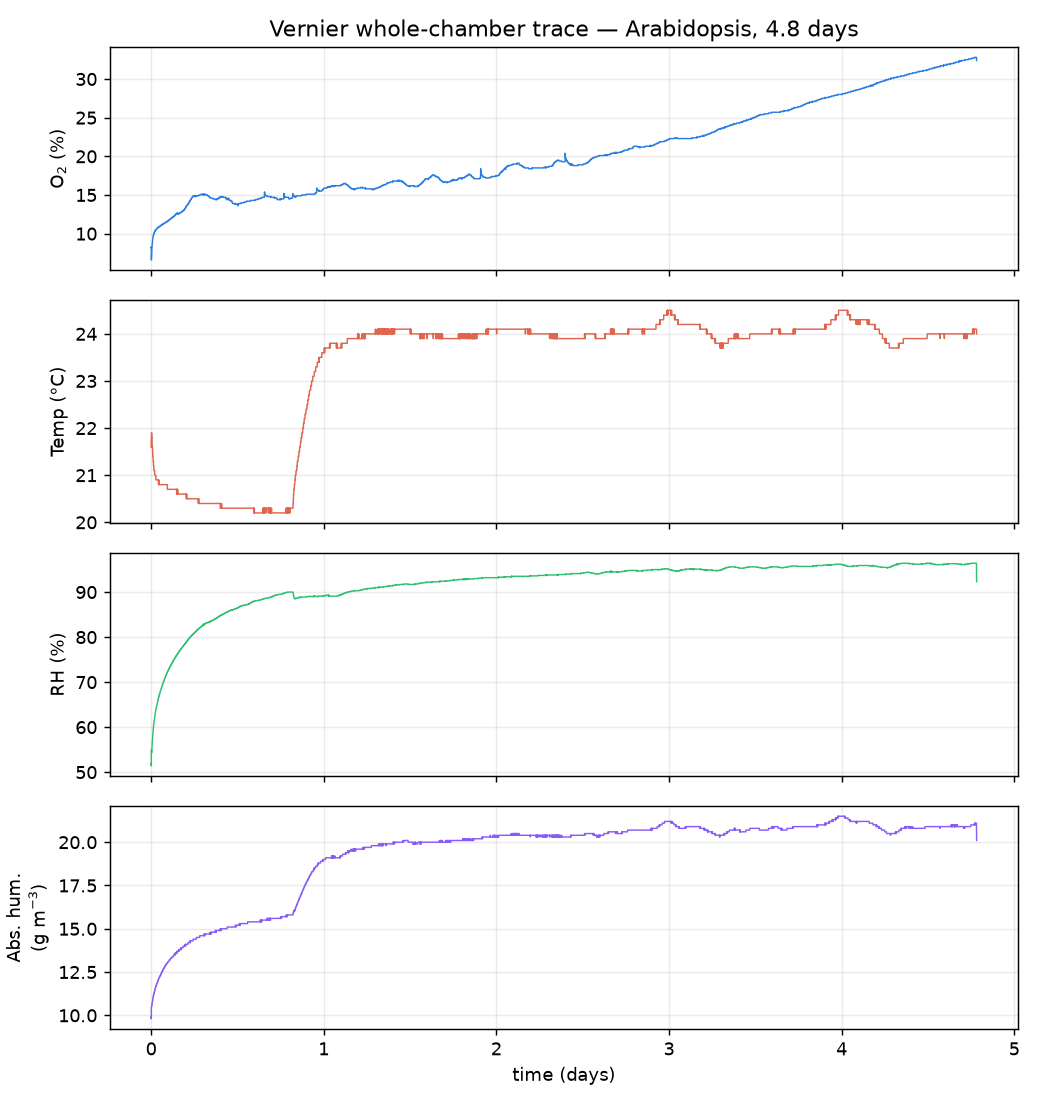
\includegraphics[width=0.46\textwidth]{F1_vernier_timeseries.png}\hfill
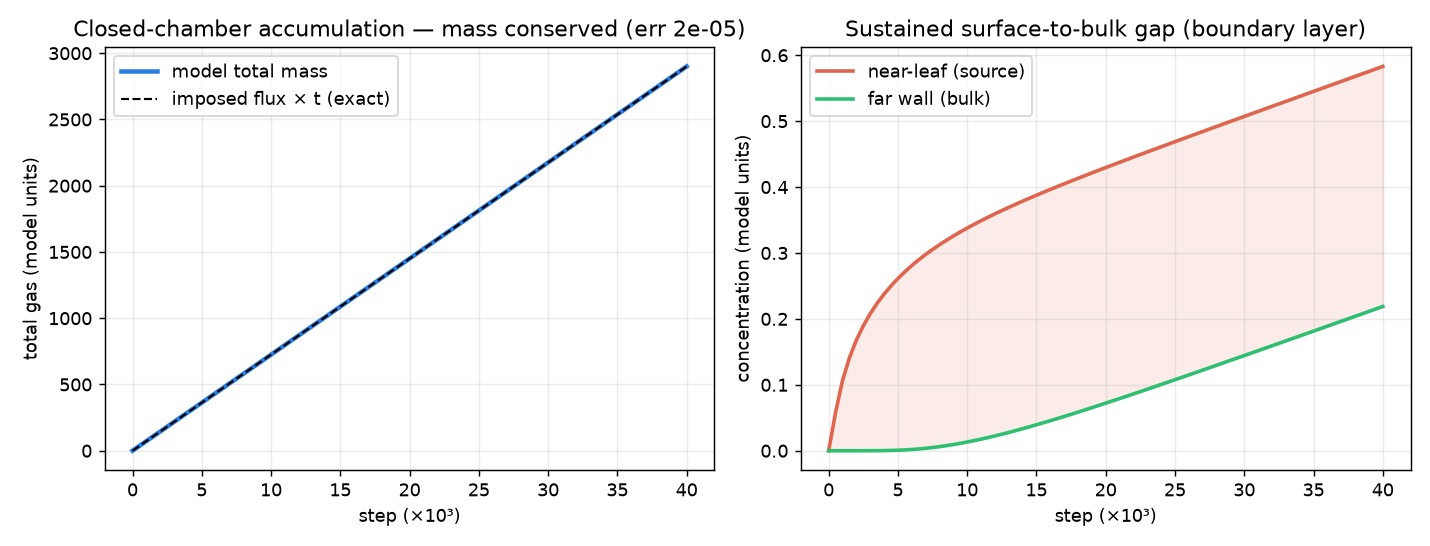
\includegraphics[width=0.52\textwidth]{F5_chamber_validation.png}
\caption{\textbf{Empirical gas-exchange anchoring and closed-chamber transport validation.}
\textbf{Left}, Measured $4.8\,\mathrm{d}$ closed-chamber Vernier trace of $\mathrm{O_2}$ ($\%$), temperature ($^\circ\mathrm{C}$), relative humidity ($\%$), and absolute humidity ($\mathrm{g\,m^{-3}}$) around \textit{Arabidopsis thaliana}, demonstrating diel photosynthetic/respiratory gas cycling (\texttt{F1\_vernier\_timeseries.png}).
\textbf{Right}, Closed-chamber lattice-Boltzmann validation (\texttt{F5\_chamber\_validation.png}): total chamber gas tracks the integrated stomatal flux to a relative mass-conservation error of $2\times 10^{-5}$, while a sustained surface-to-bulk concentration gap develops between the near-leaf fluid and the far wall.}
\label{fig:calibration_validation}
\end{figure*}

%-----------------------------------------------------------------------------
\subsection{Gravity and plant architecture control the diffusive boundary layer}\label{sec:gravity_scale}

We next evaluated steady-state gas transport (150{,}000 steps $\approx 26\,\mathrm{s}$, or 900{,}000 steps $\approx 156\,\mathrm{s}$ for the slowly diffusing $\mu g$ canopy; drift $0.00\%$ over the final $5\,\mathrm{s}$ in all cases; Supplementary Fig.~\ref{fig:s_stationarity_outlet}a and Table~\ref{tab:s_gci}) across four gravity levels---Earth ($1\,g = 9.81\,\msq$), Mars ($0.38\,g$), Moon ($0.17\,g$), and microgravity ($0\,g$)---and three geometric scales: an isolated leaf blade, an overlapping eight-leaf rosette, and a dense microgreen canopy of upright shoots spaced $3.5\,\mathrm{mm}$ apart (Fig.~\ref{fig:plumes}, Fig.~\ref{fig:grav_scale}, Table~\ref{tab:cfd_sweep}).

\begin{figure*}[tbp]
\centering
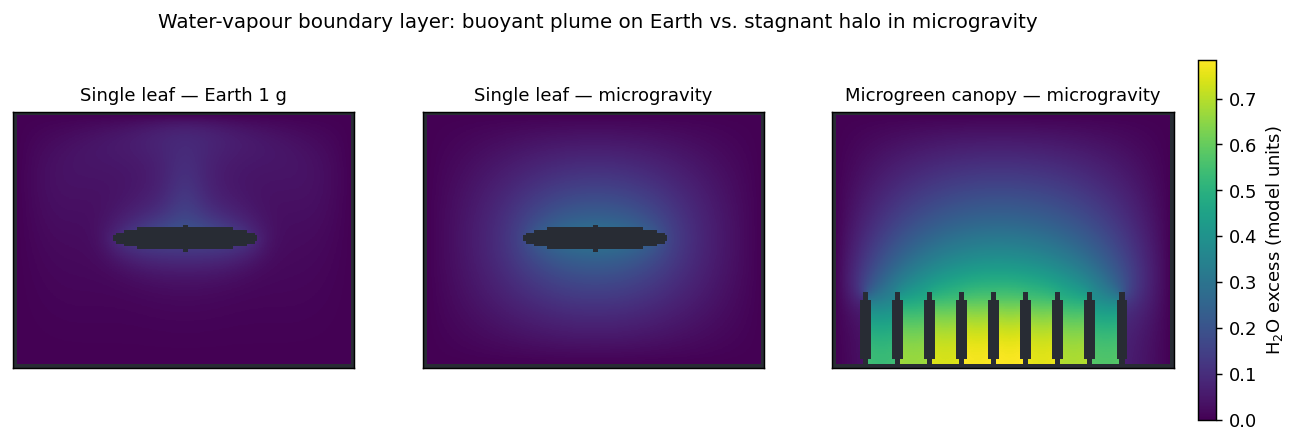
\includegraphics[width=\textwidth]{F3_plume_maps.png}
\caption{\textbf{Steady-state water-vapour boundary layers across gravity and plant architecture.}
Simulated $\mathrm{H_2O}$ concentration excess (model units) at steady state (\texttt{F3\_plume\_maps.png}). At $1\,g$ (\textbf{left}), solutal buoyancy drives an upward convective plume that thins the upper-surface boundary layer. In microgravity (\textbf{centre}), buoyant convection vanishes ($u_{\max}=0$) and a thick, symmetric diffusive halo surrounds the isolated leaf. In a microgravity microgreen canopy (\textbf{right}), overlapping diffusive halos merge between adjacent shoots, trapping stagnant air throughout the stand interior.}
\label{fig:plumes}
\end{figure*}

\begin{figure*}[tbp]
\centering
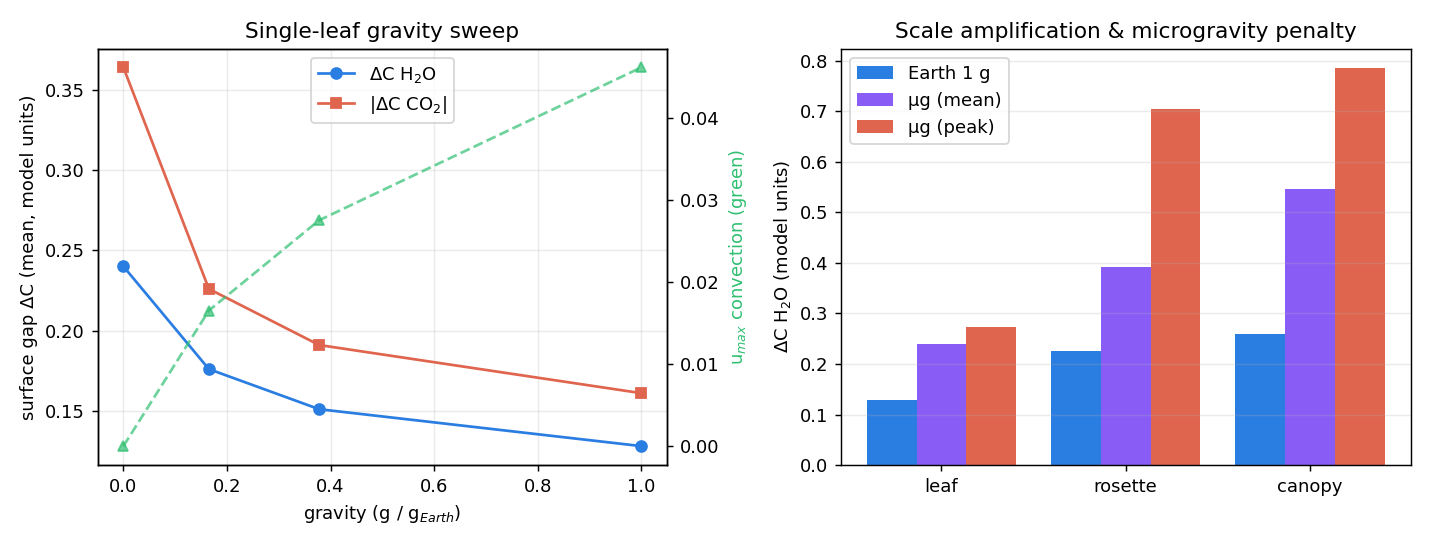
\includegraphics[width=\textwidth]{F4_gravity_scale.png}
\caption{\textbf{Gravity scaling and architectural amplification of surface gas gradients.}
\textbf{Left}, Single-leaf gravity sweep from $\mu g$ through Moon ($0.17\,g$) and Mars ($0.38\,g$) to Earth ($1\,g$): convective peak velocity $u_{\max}$ scales as $\propto\sqrt{g}$, while mean surface $\mathrm{H_2O}$ and $|\mathrm{CO_2}|$ concentration gaps steepen monotonically as gravity falls.
\textbf{Right}, Architectural amplification across isolated leaf, overlapping rosette, and microgreen canopy scales at $1\,g$ and $\mu g$ (\texttt{F4\_gravity\_scale.png}).}
\label{fig:grav_scale}
\end{figure*}

At $1\,g$, humid, $\mathrm{CO_2}$-depleted air rises off the leaf in a buoyant plume ($\mathrm{Ra}_{\mathrm{H_2O}} = 1.4\times 10^4$), sweeping the upper blade surface and maintaining an effective boundary-layer conductance of $g_{bl} = 0.997\,\molms$ and an equivalent diffusive film thickness of $\delta = D_{\mathrm{CO_2}}/g_{bl} = 0.67\,\mathrm{mm}$ ($\mathrm{Sh} = 22.4$; Table~\ref{tab:cfd_sweep}). Reducing gravity through Martian and Lunar levels weakens convective velocity as $u_{\max}\propto\sqrt{g}$ ($4.61\times 10^{-2} \to 2.75\times 10^{-2} \to 1.65\times 10^{-2} \to 0$ lattice units), causing $\delta$ to thicken monotonically to $0.79\,\mathrm{mm}$ (Mars), $0.93\,\mathrm{mm}$ (Moon), and $1.50\,\mathrm{mm}$ in microgravity ($g_{bl} = 0.443\,\molms$, a $2.25\times$ reduction; Fig.~\ref{fig:grav_scale} left).

\begin{table*}[tbp]
\caption{\textbf{Steady-state lattice-Boltzmann boundary-layer diagnostics, physical surface $\mathrm{CO_2}$/$\mathrm{O_2}$ perturbations, and closed-loop spatial assimilation across gravity and plant scales.}
Compiled from \texttt{T2\_model\_sweep.csv}, \texttt{T5\_physical\_prediction.csv}, \texttt{T12\_feedback\_spatial.csv}, and \texttt{T13\_boundary\_layer.csv}. Every scenario converged to $0.00\%$ drift in $g_{bl}$ over the final $5\,\mathrm{s}$ of simulation.}
\label{tab:cfd_sweep}
\centering
\footnotesize
\resizebox{\textwidth}{!}{%
\begin{tabular}{llccccccc}
\toprule
\textbf{Scenario} & \textbf{Gravity} & \textbf{$u_{\max}$ (lat.)} & \textbf{$g_{bl}$ ($\molms$)} & \textbf{$\delta$ ($\mathrm{mm}$)} & \textbf{$\mathrm{Sh}$} & \textbf{$\Delta\mathrm{CO_2}$ mean/peak ($\mathrm{ppm}$)} & \textbf{$\Delta\mathrm{O_2}$ mean ($\mathrm{ppm}$)} & \textbf{Closed-loop $A$ ($\%$)} \\
\midrule
Leaf $\cdot$ Earth & $1.00\,g$ & $4.61\times 10^{-2}$ & $0.997$ & $0.67$ & $22.4$ & $3.8$ / $5.9$ & $2.7$ & $98.9$ \\
Leaf $\cdot$ Mars & $0.38\,g$ & $2.75\times 10^{-2}$ & $0.841$ & $0.79$ & $18.9$ & $4.6$ / $6.8$ & $3.2$ & --- \\
Leaf $\cdot$ Moon & $0.17\,g$ & $1.65\times 10^{-2}$ & $0.712$ & $0.93$ & $16.0$ & $5.4$ / $7.8$ & $3.8$ & --- \\
Leaf $\cdot$ $\mu g$ & $0.00\,g$ & $0.00$ & $0.443$ & $1.50$ & $10.0$ & $8.7$ / $9.9$ & $5.5$ & $97.6$ \\
\midrule
Rosette $\cdot$ Earth & $1.00\,g$ & $4.60\times 10^{-2}$ & $0.540$ & $1.23$ & $16.4$ & $7.1$ / $17.1$ & $4.8$ & --- \\
Rosette $\cdot$ $\mu g$ & $0.00\,g$ & $0.00$ & $0.272$ & $2.45$ & $8.2$ & $14.2$ / $25.4$ & $8.9$ & $96.1$ \\
\midrule
Canopy $\cdot$ Earth & $1.00\,g$ & $7.19\times 10^{-2}$ & $0.133$ & $5.02$ & $1.5$ & $8.7$ / $15.3$ & $5.7$ & --- \\
Canopy $\cdot$ $\mu g$ & $0.00\,g$ & $0.00$ & $0.058$ & $11.42$ & $0.7$ & $19.8$ / $28.4$ & $12.5$ & $94.5$ \\
\bottomrule
\end{tabular}%
}
\end{table*}

Plant architecture compounds the microgravity transport penalty (Fig.~\ref{fig:grav_scale} right; Table~\ref{tab:cfd_sweep}). In an overlapping rosette, leaves shelter the central crown, reducing $g_{bl}$ from $0.540\,\molms$ on Earth to $0.272\,\molms$ in $\mu g$ ($\delta = 2.45\,\mathrm{mm}$) and elevating the peak crown $\mathrm{CO_2}$ drawdown to $25.4\,\mathrm{ppm}$ ($14.2\,\mathrm{ppm}$ mean). In a dense microgreen canopy, boundary layers of adjacent shoots merge into a stand-wide stagnant layer: $g_{bl}$ drops from $0.133\,\molms$ at $1\,g$ to $0.058\,\molms$ in $\mu g$ ($\delta = 11.42\,\mathrm{mm}$), producing a mean surface $\mathrm{CO_2}$ drawdown of $19.8\,\mathrm{ppm}$ ($28.4\,\mathrm{ppm}$ peak) and a mean $\mathrm{O_2}$ excess of $12.5\,\mathrm{ppm}$. Replacing the reference elliptical cross-section with a realistic anatomical blade outline and transverse leaf curl (\texttt{NeuraLeaf} representation; Supplementary Table~\ref{tab:s_shape_dist}) further reduced $g_{bl}$ by $3.8\text{--}5.6\%$ (outline) and $16.8\text{--}18.6\%$ (curl), with blade curl and microgravity compounding on the sheltered adaxial pocket to reach $2.6\times$ the peak $\Delta\mathrm{CO_2}$ of a flat Earth blade. Three-grid Richardson extrapolation ($0.288$, $0.192$, and $0.144\,\mathrm{mm}$) confirmed monotonic convergence with a Celik et al.~\citep{celik2008} fine-grid convergence index $\mathrm{GCI}_{\text{fine}} = 3.16\%$ at $1\,g$ and $0.87\%$ at $0\,g$ (Supplementary Table~\ref{tab:s_gci}).

%-----------------------------------------------------------------------------
\subsection{Forced ventilation reverses the microgravity penalty in a density-dependent manner}\label{sec:ventilation}

Because the microgravity boundary-layer penalty is purely transport-limited, it can be engineered away by replacing absent buoyant convection with forced airflow. Using a pressure-pinned outlet ($\rho = 1$) paired with a density-matched velocity inlet that delivers $99.6\text{--}100.9\%$ of the set mass flux across all low-Mach runs ($\mathrm{Ma}\le 0.3$; Supplementary Fig.~\ref{fig:s_stationarity_outlet}b), we swept horizontal ventilation velocity across all three plant architectures in microgravity (Fig.~\ref{fig:fan_scale}; Supplementary Fig.~\ref{fig:s_leaf_fan}).

\begin{figure*}[tbp]
\centering
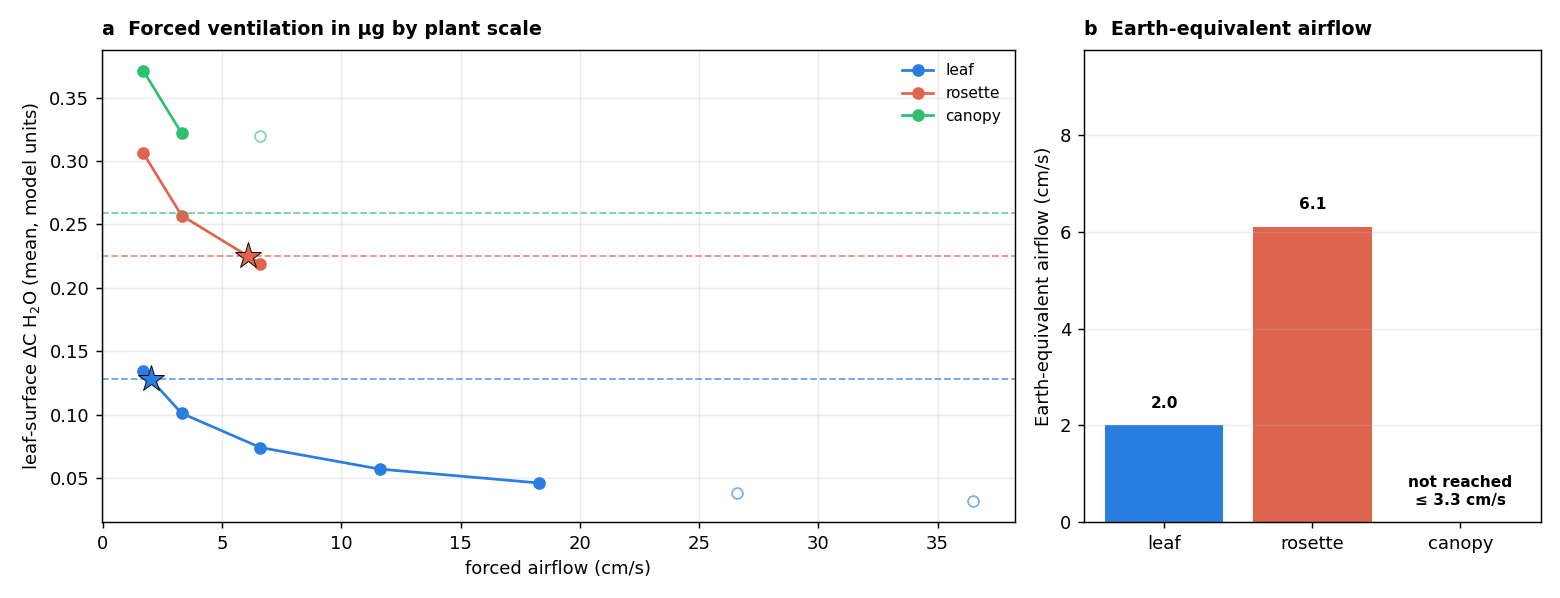
\includegraphics[width=\textwidth]{F8_fan_by_scale.png}
\caption{\textbf{Forced-ventilation requirement scales steeply with planting density.}
\textbf{a}, Steady-state surface $\mathrm{H_2O}$ concentration gap ($\Delta C_{\mathrm{H_2O}}$, model units) versus forced inlet airspeed ($\cmsu$) in microgravity across isolated leaf, rosette, and microgreen canopy scales (\texttt{F8\_fan\_by\_scale.png}). Horizontal dashed lines indicate each architecture's $1\,g$ free-convection reference; hollow symbols exceed the lattice-Boltzmann low-Mach threshold ($\mathrm{Ma}>0.3$) and are excluded from crossing interpolation.
\textbf{b}, Earth-equivalent forced airspeed required to restore $1\,g$ boundary-layer transport: $\approx 2.0\,\cmsu$ for an isolated leaf and $\approx 6.1\,\cmsu$ for a rosette ($3\times$ higher), whereas horizontal skimming flow does not restore the dense microgreen canopy within the low-Mach regime ($\le 3.3\,\cmsu$).}
\label{fig:fan_scale}
\end{figure*}

For an isolated leaf in microgravity, a horizontal airflow of only $\approx 2.0\,\cmsu$ ($\approx 2.1\,\cmsu$ for $\mathrm{CO_2}$) restores the surface concentration gap to its $1\,g$ free-convection value (Fig.~\ref{fig:fan_scale}a,b; \texttt{T6\_forced\_airflow.csv}). However, extending the sweep to denser architectures reveals a critical scaling law for hardware design: an overlapping rosette requires $\approx 6.1\,\cmsu$ ($3\times$ higher airspeed) to achieve Earth parity, and even when VEGGIE-level airflow ($\sim 8\,\cmsu$) restores the rosette's \emph{mean} surface gap ($|\Delta C_{\mathrm{CO_2}}| = 0.289$ vs.\ $0.298$ at $1\,g$), it leaves highly uneven spatial ventilation across the sheltered crown (coefficient of variation $\mathrm{CoV} = 0.66$ vs.\ $0.49$ at $1\,g$; Supplementary Table~\ref{tab:s_shape_dist}). For the dense microgreen canopy, horizontal side-to-side airflow skims across the top of the shoot tips while inter-shoot air remains stagnant; its surface gap remains above the $1\,g$ level across the solver's valid low-Mach regime ($\le 3.3\,\cmsu$). Thus, a single ventilation speed tuned on sparse seedlings systematically under-ventilates a dense stand.

%-----------------------------------------------------------------------------
\subsection{Spaceflight growth hardware as boundary conditions: illuminated sealed canisters are $\mathrm{CO_2}$-starvation chambers}\label{sec:hardware}

Whereas gravity and fan speed govern the sub-millimetre boundary layer ($C_a \to C_s$), the growth container governs the bulk enclosure atmosphere ($C_{\text{cabin}} \to C_a$). We modelled the three primary ISS plant-growth hardware classes both as lattice-Boltzmann boundary conditions (zero-flux walls for hermetically sealed BRIC, semi-permeable relaxing walls for micropore-taped CARA, and forced inlet/outlet channel flow for VEGGIE; Supplementary Fig.~\ref{fig:s_hw_scale}) and as coupled zero-dimensional (0-D) headspace mass balances over a $12\,\mathrm{h}$ photoperiod (Fig.~\ref{fig:hardware}; Supplementary Table~\ref{tab:s_enclosure_params}).

\begin{figure*}[tbp]
\centering
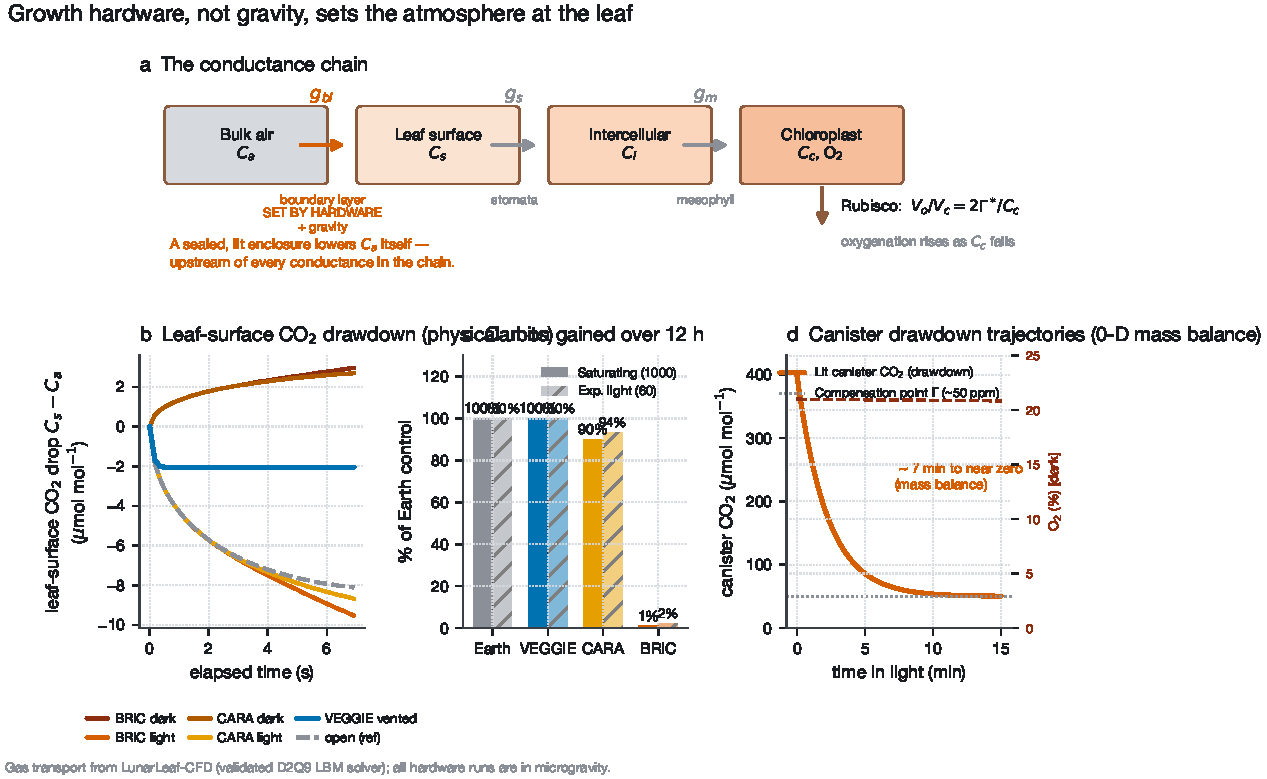
\includegraphics[width=\textwidth]{fig01_hardware_atmosphere.pdf}
\caption{\textbf{Growth hardware, not gravity, sets the bulk atmosphere at the leaf.}
\textbf{a}, Series conductance chain from cabin air across the enclosure seal, boundary layer ($g_{bl}$, the sole gravity-dependent step), stomata ($g_s$), and mesophyll ($g_m$) to Rubisco ($C_c$).
\textbf{b}, Lattice-Boltzmann leaf-surface $\mathrm{CO_2}$ drawdown ($C_s - C_a$, $\mu\mathrm{mol\,mol^{-1}}$) over elapsed physical time (\texttt{T7\_hardware\_timeseries.csv}), showing identical surface diffusive penalties for BRIC and CARA in microgravity while VEGGIE forced airflow thins the boundary layer $\sim 4\times$.
\textbf{c}, Integrated $12\,\mathrm{h}$ photoperiod carbon gain ($\%$ of unenclosed $1\,g$ control) under experimental ($60\,\ums$) and saturating ($1000\,\ums$) irradiance (\texttt{T11\_photosynthesis\_feedback.csv}).
\textbf{d}, Dynamic 0-D canister mass-balance trajectories (\texttt{T8\_enclosure\_timescales.csv}), showing exhaustion of headspace $\mathrm{CO_2}$ to the compensation point within $\sim 7\,\mathrm{min}$ in illuminated sealed BRIC canisters and gradual $\mathrm{O_2}$ depletion toward hypoxia ($\sim 6.5\,\mathrm{d}$) in dark canisters (\texttt{fig01\_hardware\_atmosphere.pdf}).}
\label{fig:hardware}
\end{figure*}

The two scales of transport separate cleanly across the three hardware classes:
\begin{itemize}
    \item \textbf{BRIC (hermetically sealed)}: With zero gas exchange across the canister wall, plant metabolism drives runaway drift of the small headspace ($30\,\mathrm{mL}$ air over $3\,\mathrm{cm^2}$ leaf area; Fig.~\ref{fig:hardware}d). In the dark, respiratory $\mathrm{CO_2}$ reaches $1\%$ ($10{,}000\,\mathrm{ppm}$) in $\approx 9\,\mathrm{h}$ and $\mathrm{O_2}$ falls from $21\%$ to hypoxic $5\%$ in $\approx 6.5\,\mathrm{d}$. In the light, the $\sim 400\,\mathrm{ppm}$ of headspace $\mathrm{CO_2}$ ($\approx 0.5\,\mu\mathrm{mol}$ total carbon) is fixed by photosynthesis in \textbf{$\approx 7\,\mathrm{min}$}. Once coupled to $\mathrm{CO_2}$-limited assimilation, headspace $\mathrm{CO_2}$ collapses to the compensation point ($\Gamma\approx 50\,\mathrm{ppm}$) within minutes and remains pinned there for the rest of the photoperiod, reducing $12\,\mathrm{h}$ cumulative carbon gain to \textbf{$1\%$} of an unenclosed Earth control (Fig.~\ref{fig:hardware}c). Sensitivity sweeps across headspace volume ($15\text{--}60\,\mathrm{mL}$), leaf area ($1\text{--}10\,\mathrm{cm^2}$), irradiance ($60\text{--}1000\,\ums$), and cabin $\mathrm{CO_2}$ ($400\text{--}1200\,\mathrm{ppm}$) confirm that rapid $\mathrm{CO_2}$ starvation is an invariant property of sealed illuminated canisters ($0.13\text{--}11.7\%$ 12\,h carbon gain across the entire parameter envelope; Supplementary Table~\ref{tab:s_enclosure_sens}).
    \item \textbf{CARA (gas-permeable micropore surgical tape)}: Diffusive exchange across the taped lid and perimeter (effective permeance $0.006\,\molms$) resupplies $\mathrm{CO_2}$ from the spacecraft cabin, sustaining \textbf{$\approx 90\text{--}95\%$} of Earth $12\,\mathrm{h}$ carbon gain (Fig.~\ref{fig:hardware}c; Supplementary Table~\ref{tab:s_enclosure_sens}). Crucially, however, passive tape permeance does not generate convective flow inside the dish: in microgravity, the leaf-surface boundary-layer gradient inside CARA is indistinguishable from that of a sealed BRIC dish (Fig.~\ref{fig:hardware}b; Supplementary Fig.~\ref{fig:s_hw_scale}). Thus, CARA solves the \emph{enclosure-atmosphere} problem while leaving the \emph{microgravity boundary-layer} problem intact.
    \item \textbf{VEGGIE (actively ventilated)}: Forced air circulation simultaneously pins the bulk atmosphere to cabin $\mathrm{CO_2}$ and thins the leaf boundary layer, cutting the surface concentration gap $\sim 4\times$ relative to unventilated dishes (Fig.~\ref{fig:hardware}b) and sustaining \textbf{$\approx 100\%$} of Earth $12\,\mathrm{h}$ carbon gain (Fig.~\ref{fig:hardware}c).
\end{itemize}

Simulations inside exact two-dimensional cross-sections of the flight Petri dishes ($60\,\mathrm{mm}$ round BRIC with $7.4\,\mathrm{mm}$ headspace above agar; $120\,\mathrm{mm}$ square CARA with $9.8\,\mathrm{mm}$ headspace; Supplementary Figs.~\ref{fig:s_real_dishes}--\ref{fig:s_dish_feedback} and Table~\ref{tab:s_real_dish}) revealed an additional geometric constraint: because the shallow $7\text{--}10\,\mathrm{mm}$ dish headspace suppresses vertical convective plumes even at $1\,g$, $g_{bl}$ inside a shallow Petri dish at $1\,g$ is already reduced to $\approx 0.25\,\molms$, narrowing the $1\,g/\mu g$ ratio inside the dish to $1.25\text{--}1.8\times$. Moreover, when transpiration is coupled to headspace humidity saturation inside a sealed BRIC dish (\texttt{T20}--\texttt{T22}), the headspace saturates within $1\text{--}2\,\mathrm{min}$, shutting down transpirational buoyancy at $1\,g$ so that the $1\,g$ and $0\,g$ boundary layers converge within minutes (Supplementary Fig.~\ref{fig:s_dish_feedback}). Because enclosure $\mathrm{CO_2}$ drawdown is a mass balance determined by leaf area and headspace volume, under symmetric thermal and sealing conditions \textbf{it occurs in the $1\,g$ ground control just as rapidly as in spaceflight}. Consequently, canister carbon starvation cancels out of a standard flight-versus-ground differential contrast, but shifts the physiological baseline of both arms into severe carbon depletion.

%-----------------------------------------------------------------------------
\subsection{Coupling CFD transport to Rubisco kinetics: enclosure drawdown dominates and converges the gravity gap}\label{sec:fvcb}

To quantify how boundary-layer conductance ($g_{bl}$) and enclosure $\mathrm{CO_2}$ ($C_a$) jointly regulate photosynthetic metabolism, we coupled the steady-state CFD $g_{bl}$ table (\texttt{T13\_boundary\_layer.csv}) to a Farquhar--von Caemmerer--Berry (FvCB) $\mathrm{C_3}$ biochemical model \citep{farquhar1980} parameterized with \textit{in vivo} \textit{Arabidopsis} Rubisco and electron-transport kinetics \citep{bernacchi2001,bernacchi2003} (Supplementary Table~\ref{tab:s_fvcb_params}), solving recursively for the supply-equals-demand chloroplastic $\mathrm{CO_2}$ concentration $C_c$ and propagating the CFD-predicted surface $\mathrm{O_2}$ build-up ($\Delta\mathrm{O_2} = 2.7\text{--}12.5\,\mathrm{ppm}$) into local $\Gamma^*$ (Fig.~\ref{fig:fvcb}, Table~\ref{tab:operating}).

\begin{figure*}[tbp]
\centering
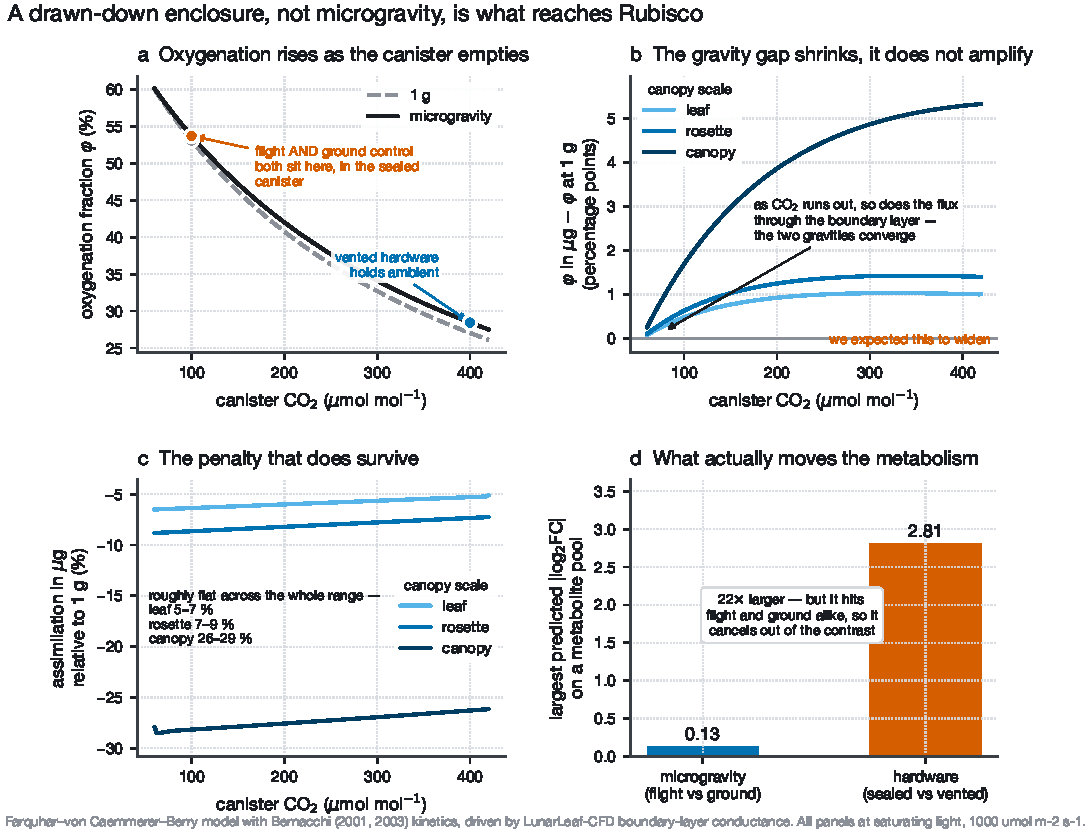
\includegraphics[width=\textwidth]{fig02_fvcb_operating_points.pdf}
\caption{\textbf{Coupled CFD--FvCB Rubisco operating points: enclosure drawdown dominates and converges the microgravity boundary-layer gap.}
\textbf{a}, Rubisco oxygenation fraction $\varphi = V_o/(V_o+V_c)$ as a function of canister $\mathrm{CO_2}$ ($C_a$) at experimental irradiance ($60\,\ums$, OSD-522; solid curves) and saturating irradiance ($1000\,\ums$; dotted curves) for $1\,g$ (blue) and $\mu g$ (vermilion) rosette conductances (\texttt{fig02\_fvcb\_operating\_points.pdf}).
\textbf{b}, The microgravity-minus-ground difference in oxygenation ($\Delta\varphi_{\mu g - 1g}$) shrinks toward zero as canister $\mathrm{CO_2}$ is drawn down toward the compensation point.
\textbf{c}, Relative microgravity assimilation deficit $(A_{1g}-A_{\mu g})/A_{1g}$ across leaf, rosette, and canopy scales at $Q = 60$ and $1000\,\ums$ (\texttt{T13\_light\_sensitivity.tsv}).
\textbf{d}, Magnitude comparison of predicted log$_2$ metabolite pool shifts: the sealed-versus-ventilated hardware effect is $22\times$ larger than the flight-versus-ground microgravity effect.}
\label{fig:fvcb}
\end{figure*}

\begin{table*}[tbp]
\caption{\textbf{Modelled CFD--FvCB operating points at experimental ($60\,\ums$) and saturating ($1000\,\ums$) irradiance.}
Shown for rosette architecture ($g_{bl} = 0.540\,\molms$ at $1\,g$; $0.272\,\molms$ in $\mu g$). $C_a$ and $C_c$ in $\mu\mathrm{mol\,mol^{-1}}$; net assimilation $A$ and photorespiration $R_p = 0.5\,V_o$ in $\ums$; oxygenation fraction $\varphi = V_o/(V_o+V_c)$ in $\%$ (\texttt{T04\_photorespiration\_vs\_gravity.csv}, \texttt{T05\_operating\_points.tsv}, \texttt{T13\_light\_sensitivity.tsv}).}
\label{tab:operating}
\centering
\footnotesize
\resizebox{\textwidth}{!}{%
\begin{tabular}{llcccccc}
\toprule
\textbf{Experimental arm} & \textbf{Irradiance $Q$ ($\ums$)} & \textbf{$g_{bl}$ ($\molms$)} & \textbf{$C_a$ ($\mathrm{ppm}$)} & \textbf{$C_c$ ($\mathrm{ppm}$)} & \textbf{$\varphi$ ($\%$)} & \textbf{$A$ ($\ums$)} & \textbf{$R_p$ ($\ums$)} \\
\midrule
Ventilated control ($\mu g$) & $60$ (BRIC-LED) & $0.272$ & $400$ & $334.6$ & $18.0$ & $4.90$ & $0.68$ \\
Sealed ground ($1\,g$) & $60$ (BRIC-LED) & $0.540$ & $100$ & $88.2$ & $45.8$ & $0.94$ & $0.97$ \\
Sealed flight ($\mu g$) & $60$ (BRIC-LED) & $0.272$ & $100$ & $87.2$ & $46.2$ & $0.88$ & $0.94$ \\
\midrule
Ventilated Earth ($1\,g$) & $1000$ (saturating) & $0.540$ & $400$ & $230.7$ & $27.0$ & $16.62$ & $4.09$ \\
Ventilated flight ($\mu g$) & $1000$ (saturating) & $0.272$ & $400$ & $215.0$ & $28.5$ & $15.40$ & $4.16$ \\
Sealed ground ($1\,g$) & $1000$ (saturating) & $0.540$ & $100$ & $75.5$ & $53.1$ & $2.40$ & $2.12$ \\
Sealed flight ($\mu g$) & $1000$ (saturating) & $0.272$ & $100$ & $73.6$ & $53.7$ & $2.20$ & $2.03$ \\
\bottomrule
\end{tabular}%
}
\end{table*}

At ambient $\mathrm{CO_2}$ ($400\,\mathrm{ppm}$) and saturating light ($1000\,\ums$), dropping from $1\,g$ to $\mu g$ lowers chloroplastic $C_c$ from $238.9$ to $227.0\,\mathrm{ppm}$ in an isolated leaf ($A$: $17.25 \to 16.34\,\ums$, a $5.3\%$ deficit), from $230.7$ to $215.0\,\mathrm{ppm}$ in a rosette ($A$: $16.62 \to 15.40\,\ums$, a $7.3\%$ deficit), and from $189.2$ to $149.3\,\mathrm{ppm}$ in a dense canopy ($A$: $13.30 \to 9.80\,\ums$, a $26.3\%$ deficit; $\varphi$ rising from $31.1\%$ to $36.4\%$). At the lower irradiance used in BRIC-LED flight OSD-522 ($Q = 60\,\ums$), RuBP regeneration ($A_j$) limits assimilation and the microgravity deficit at ambient $\mathrm{CO_2}$ is smaller: $<3\%$ at leaf and rosette scale and up to $11\%$ in a dense canopy (Fig.~\ref{fig:fvcb}c).

By contrast, drawing the canister headspace down from $400\,\mathrm{ppm}$ to $100\,\mathrm{ppm}$ in a sealed lit BRIC canister shifts the leaf dramatically along its $\mathrm{CO_2}$ response curve: at $Q = 60\,\ums$, the Rubisco oxygenation fraction $\varphi$ jumps from \textbf{$18.0\%$ to $46.2\%$}, and net assimilation $A$ drops more than five-fold from $4.90$ to $0.88\,\ums$ ($53.7\%$ oxygenation at $Q = 1000\,\ums$; Fig.~\ref{fig:fvcb}a, Table~\ref{tab:operating}). Crucially, this coupling refuted our own initial hypothesis. We had hypothesized that canister $\mathrm{CO_2}$ drawdown would \emph{amplify} the microgravity boundary-layer penalty. Instead, the $1\,g$ and $\mu g$ curves \textbf{converge} as $C_a$ approaches $\Gamma^*$ (Fig.~\ref{fig:fvcb}b): because the concentration drop across the boundary layer is $\Delta C_{bl} = A/g_{bl}$, as $A\to 0$ near the compensation point, the flux across the boundary layer vanishes and gravity has nothing left to impede. Across the 21 modelled metabolic pools, the sealed-versus-ventilated enclosure effect is \textbf{$22\times$ larger} than the flight-versus-ground microgravity effect (Fig.~\ref{fig:fvcb}d).

%-----------------------------------------------------------------------------
\subsection{The OSDR plant metabolomics gap and a falsifiable 21-compound hypothesis scaffold}\label{sec:metabolome}

Multi-omics pathway integration across central carbon and photorespiratory metabolism requires metabolite measurements alongside transcriptomics and proteomics. We queried all 567 studies in the NASA Open Science Data Repository (\texttt{T03\_osdr\_metabolomics\_census.tsv}; Supplementary Table~\ref{tab:s_osdr_census}) and identified 12 studies with metabolite-profiling assays: all 12 are mammalian (\textit{Homo sapiens}, \textit{Mus musculus}, \textit{Rattus norvegicus}) or microbial. \textbf{No plant spaceflight study in NASA OSDR contains a metabolome.}

\begin{figure*}[tbp]
\centering
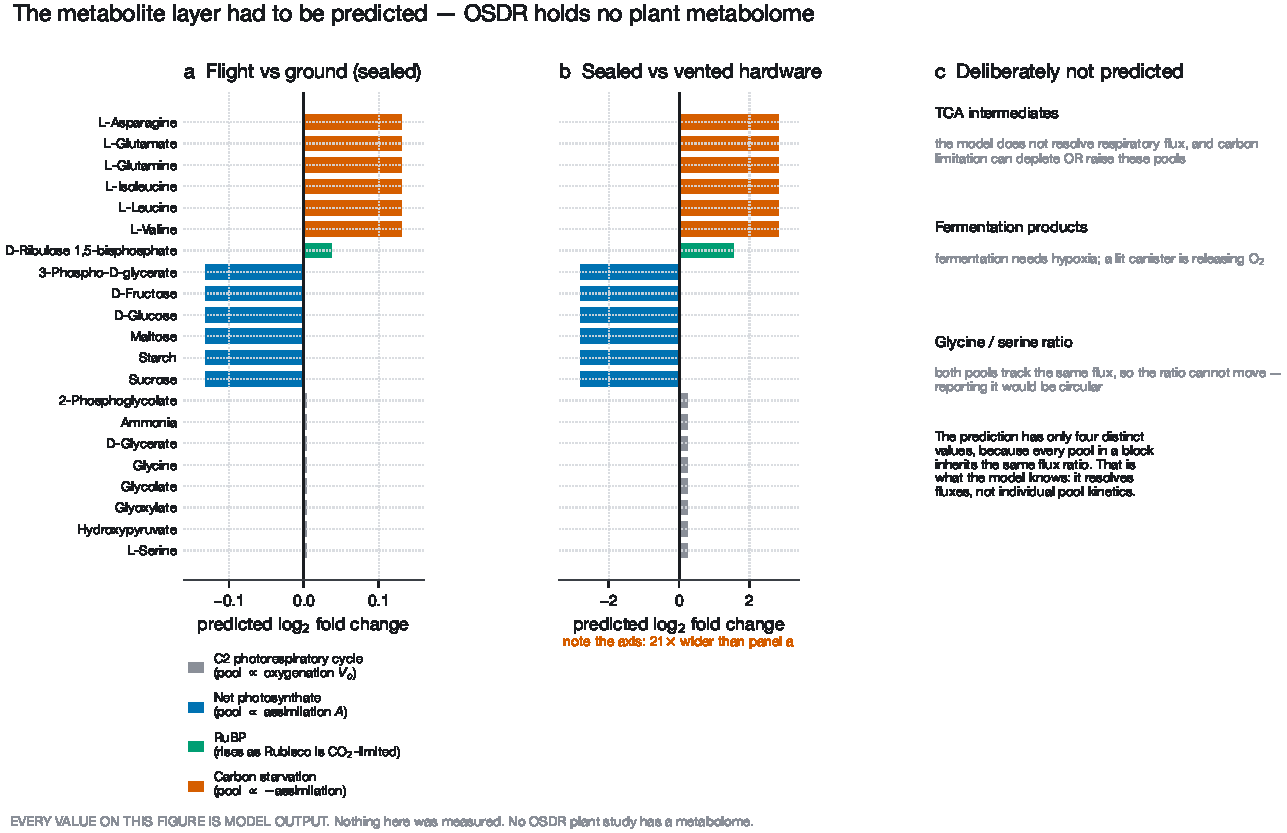
\includegraphics[width=\textwidth]{fig03_predicted_metabolome.pdf}
\caption{\textbf{The 21-compound predicted metabolite hypothesis scaffold.}
Quasi-steady-state flux-propagated log$_2$ fold-change predictions ($\log_2(P_{\text{arm1}}/P_{\text{arm2}}) = \log_2(J_{\text{arm1}}/J_{\text{arm2}})$) across Tier 1 stoichiometric intermediates (driven by $V_o$ and $A$) and Tier 2 carbon-starvation / RuBP pools (driven by $-C_c$ and $-A$), comparing the flight-versus-ground microgravity contrast against the sealed-versus-ventilated enclosure contrast (\texttt{T06\_predicted\_compounds.tsv}, \texttt{fig03\_predicted\_metabolome.pdf}). All values are explicitly labelled as model output.}
\label{fig:metabolome}
\end{figure*}

To enable trimodal pathway topology testing and provide a concrete target list for future chemical profiling of archived flight tissues, we formulated a transparent 21-compound predicted metabolite layer (Fig.~\ref{fig:metabolome}; Supplementary Table~\ref{tab:s_metabolite_mapping}) by propagating the FvCB fluxes under quasi-steady state ($\log_2(P_1/P_2) = \log_2(J_1/J_2)$): eight $\mathrm{C_2}$ photorespiratory intermediates driven by $V_o$ (2-phosphoglycolate, glycolate, glyoxylate, glycine, L-serine, hydroxypyruvate, D-glycerate, ammonia), six photosynthetic carbon products driven by $A$ (3-phosphoglycerate, sucrose, D-glucose, D-fructose, maltose, starch), RuBP driven by $-C_c$, and six amino-acid carbon-starvation markers driven by $-A$ (L-asparagine, branched-chain amino acids L-valine, L-leucine, L-isoleucine, and nitrogen-remobilization hubs L-glutamine and L-glutamate). Every table, figure, and interactive chart in the repository explicitly labels this layer as model prediction rather than measurement.

%-----------------------------------------------------------------------------
\subsection{Testing against OSD-522 (BRIC-LED): the coupled model calls eight of nine transcriptome gene sets while ER unfolded protein response dominates globally}\label{sec:osd522}

We tested the model's predictions against NASA OSDR study OSD-522 (BRIC-LED-001) \citep{osd522}, which grew \textit{Arabidopsis thaliana} Col-0 shoots for $11\,\mathrm{d}$ inside sealed BRIC-LED canisters under $60\,\ums$ illumination ($n = 6$ flight vs.\ $n = 6$ ground biological replicates) and provides paired RNA-seq and TMT quantitative proteomics from the same experiment (Fig.~\ref{fig:osd522_blind}). Differential expression analysis of the shoot RNA-seq counts with PyDESeq2 \citep{pydeseq2} (\texttt{T01\_osd522\_transcriptome.tsv}) yielded $1{,}795$ differentially expressed genes (DEGs) at Benjamini--Hochberg $\mathrm{FDR}<0.05$ out of $19{,}325$ tested loci ($1{,}658$ low-count loci received $\mathrm{NA}$ adjusted $p$-values via standard DESeq2 independent filtering; Fig.~\ref{fig:osd522_blind}a,b). Processing the deposited soluble and membrane shoot proteomics (\texttt{T02\_osd522\_proteome.tsv}) yielded ratios for $5{,}160$ proteins ($4{,}296$ co-measured with RNA-seq; Fig.~\ref{fig:osd522_blind}c,d).

\begin{figure*}[tbp]
\centering
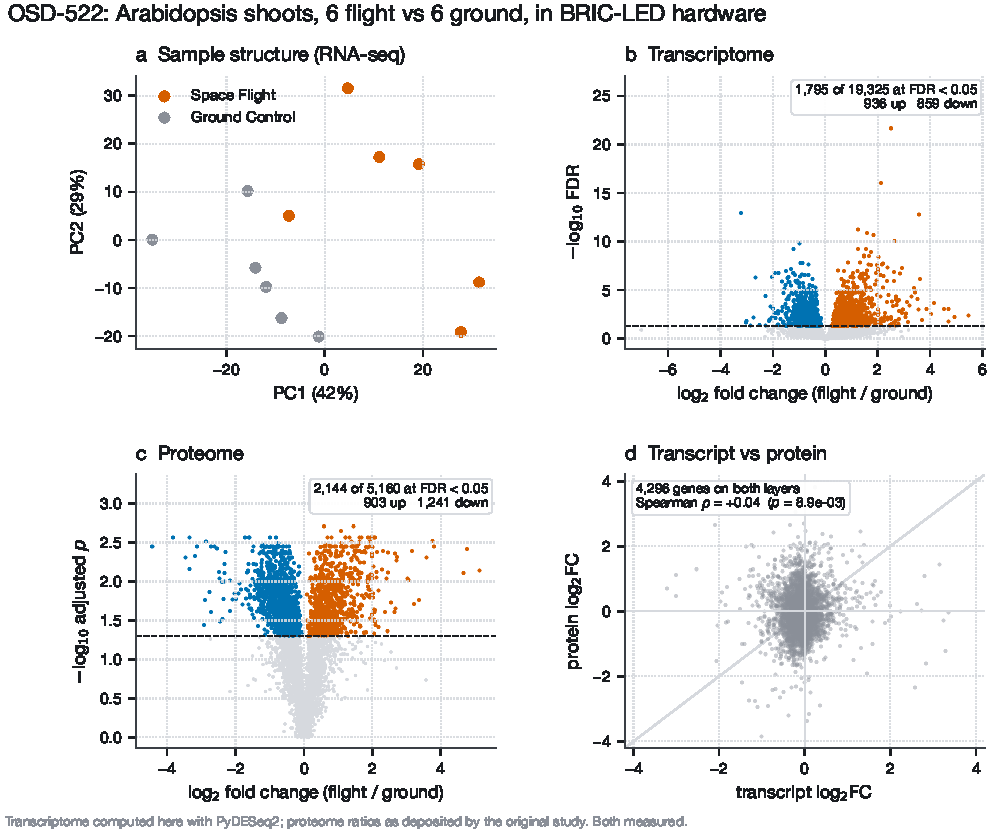
\includegraphics[width=0.49\textwidth]{fig04_osd522_omics.pdf}\hfill
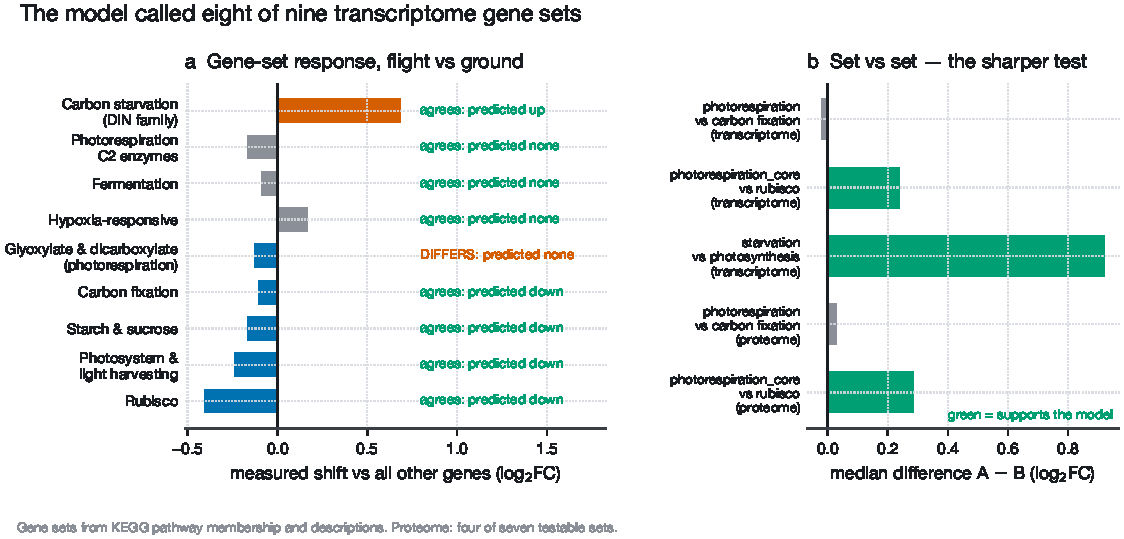
\includegraphics[width=0.49\textwidth]{fig05_blind_test.pdf}
\caption{\textbf{OSD-522 (BRIC-LED) shoot multi-omics profiling and directional gene-set falsification test.}
\textbf{Left} (\texttt{fig04\_osd522\_omics.pdf}): \textbf{a}, Principal component analysis of OSD-522 shoot RNA-seq libraries ($6$ flight vs.\ $6$ ground). \textbf{b}, Transcriptome volcano plot ($1{,}795$ DEGs at $\mathrm{FDR}<0.05$). \textbf{c}, Shoot proteome volcano plot ($5{,}160$ proteins). \textbf{d}, Transcript-versus-protein $\log_2\mathrm{FC}$ comparison across $4{,}296$ co-measured loci.
\textbf{Right} (\texttt{fig05\_blind\_test.pdf}): \textbf{a}, Directional predictions versus observed Mann--Whitney median $\log_2\mathrm{FC}$ shifts across nine KEGG-derived gene sets in the transcriptome (8 of 9 matched) and proteome (4 of 7 matched). \textbf{b}, Set-versus-set relative contrasts demonstrating selective maintenance of core photorespiratory enzymes above Rubisco ($+0.239$ transcriptome, $p = 6.8\times 10^{-3}$; $+0.285$ proteome, $p = 4.9\times 10^{-2}$) and strong induction of \textit{DIN} carbon-starvation markers over photosynthetic machinery ($+0.923$, $p = 5.3\times 10^{-6}$).}
\label{fig:osd522_blind}
\end{figure*}

Scoring the transcriptome and proteome against nine pre-specified KEGG and literature gene sets (\texttt{scripts/genesets.py}, \texttt{T07\_falsification\_osd522.tsv}; Fig.~\ref{fig:osd522_blind} right, Table~\ref{tab:falsification}) confirmed \textbf{eight of nine directional calls in the transcriptome} and \textbf{four of seven in the proteome}:
\begin{enumerate}
    \item \textbf{Photosynthetic apparatus repression}: Light-harvesting and photosystem subunits (\texttt{ath00195}/\texttt{ath00196}) fell significantly in both the transcriptome (median shift $-0.238$, $p = 3.8\times 10^{-6}$) and proteome ($-0.820$, $p = 5.0\times 10^{-4}$).
    \item \textbf{Rubisco and Calvin-cycle repression}: Rubisco subunits (\texttt{RBCS1A--3B}, \texttt{RBCL}) fell strongly in the transcriptome ($-0.403$, $p = 4.5\times 10^{-3}$; proteome $-0.390$, $p = 0.062$), alongside broader photosynthetic carbon fixation (\texttt{ath00710}; transcriptome $-0.105$, $p = 1.3\times 10^{-4}$) and starch/sucrose metabolism (\texttt{ath00500}; transcriptome $-0.165$, $p = 3.5\times 10^{-6}$).
    \item \textbf{Carbon-starvation induction}: Classic dark-inducible / carbon-starvation markers (\textit{DIN6/ASN1}, \textit{DIN1}, \textit{DIN10}, \textit{BCAT2}) rose sharply in the transcriptome ($+0.685$, $p = 2.6\times 10^{-3}$).
    \item \textbf{Absence of bulk photorespiratory or hypoxic induction, but selective maintenance of $\mathrm{C_2}$ enzymes over Rubisco}: Because canister $\mathrm{CO_2}$ starvation occurs in both flight and ground canisters (and gravity converges at low $\mathrm{CO_2}$), the model predicted no strong net induction of core photorespiratory enzymes (\texttt{photorespiration\_core}: $p = 0.092$ transcriptome, $p = 0.414$ proteome; \texttt{MATCH}), fermentation ($p = 0.596$ transcriptome, $p = 0.067$ proteome; \texttt{MATCH}), or core hypoxia markers ($p = 0.248$ transcriptome; \texttt{MATCH}). Crucially, however, in set-versus-set contrasts that control for global transcriptional depression of plastid genes, core photorespiratory enzymes sat significantly \textbf{above Rubisco} in both the transcriptome ($+0.239\,\log_2\mathrm{FC}$, $p = 6.8\times 10^{-3}$) and the proteome ($+0.285\,\log_2\mathrm{FC}$, $p = 4.9\times 10^{-2}$; Table~\ref{tab:falsification}B), and carbon-starvation markers sat $+0.923\,\log_2\mathrm{FC}$ above the photosynthetic apparatus ($p = 5.3\times 10^{-6}$).
\end{enumerate}

\begin{table*}[tbp]
\caption{\textbf{OSD-522 (BRIC-LED) multi-omics falsification scorecard across KEGG-derived gene sets and set-versus-set contrasts.}
Mann--Whitney $U$ shifts (gene-set median minus genome-wide background median) and two-sided $p$-values across the shoot transcriptome ($19{,}325$ loci) and shoot proteome ($5{,}160$ proteins) from \texttt{T07\_falsification\_osd522.tsv}.}
\label{tab:falsification}
\centering
\footnotesize
\resizebox{\textwidth}{!}{%
\begin{tabular}{llcccccc}
\toprule
\textbf{Gene set / Contrast} & \textbf{Layer} & \textbf{$n$} & \textbf{Median $\log_2\mathrm{FC}$} & \textbf{Shift vs.\ bg} & \textbf{$p$-value} & \textbf{Predicted} & \textbf{Verdict} \\
\midrule
\multicolumn{8}{l}{\textbf{A. Single gene-set directional tests (vs.\ genome background)}} \\
\midrule
Photosynthesis apparatus & Transcriptome & $31$ & $-0.215$ & $-0.238$ & $3.8\times 10^{-6}$ & Down & Match \\
Rubisco subunits & Transcriptome & $5$ & $-0.381$ & $-0.403$ & $4.5\times 10^{-3}$ & Down & Match \\
Carbon fixation (\texttt{ath00710}) & Transcriptome & $66$ & $-0.082$ & $-0.105$ & $1.3\times 10^{-4}$ & Down & Match \\
Starch \& sucrose (\texttt{ath00500}) & Transcriptome & $142$ & $-0.142$ & $-0.165$ & $3.5\times 10^{-6}$ & Down & Match \\
Carbon starvation (\textit{DIN}) & Transcriptome & $5$ & $+0.708$ & $+0.685$ & $2.6\times 10^{-3}$ & Up & Match \\
Photorespiration core ($\mathrm{C_2}$) & Transcriptome & $13$ & $-0.142$ & $-0.164$ & $0.092$ & None & Match \\
Glyoxylate/dicarboxylate (\texttt{ath00630}) & Transcriptome & $76$ & $-0.102$ & $-0.125$ & $3.2\times 10^{-4}$ & None & Mismatch (Down) \\
Fermentation & Transcriptome & $6$ & $-0.067$ & $-0.090$ & $0.596$ & None & Match \\
Hypoxia responsive & Transcriptome & $3$ & $+0.191$ & $+0.169$ & $0.248$ & None & Match \\
\midrule
Photosynthesis apparatus & Proteome & $19$ & $-0.920$ & $-0.820$ & $5.0\times 10^{-4}$ & Down & Match \\
Rubisco subunits & Proteome & $3$ & $-0.490$ & $-0.390$ & $0.062$ & Down & Mismatch ($p=0.06$) \\
Carbon fixation (\texttt{ath00710}) & Proteome & $55$ & $+0.050$ & $+0.150$ & $0.194$ & Down & Mismatch \\
Starch \& sucrose (\texttt{ath00500}) & Proteome & $68$ & $-0.195$ & $-0.095$ & $0.133$ & Down & Mismatch \\
Photorespiration core ($\mathrm{C_2}$) & Proteome & $10$ & $-0.205$ & $-0.105$ & $0.414$ & None & Match \\
Glyoxylate/dicarboxylate (\texttt{ath00630}) & Proteome & $55$ & $+0.080$ & $+0.190$ & $0.296$ & None & Match \\
Fermentation & Proteome & $3$ & $+0.510$ & $+0.610$ & $0.067$ & None & Match \\
\midrule
\multicolumn{8}{l}{\textbf{B. Set-versus-set relative contrasts (immune to global plastid depression)}} \\
\midrule
Photorespiration core vs.\ Rubisco & Transcriptome & $13$ vs.\ $5$ & $-0.142$ vs.\ $-0.381$ & $+0.239$ & $6.8\times 10^{-3}$ & A $>$ B & Supports \\
Photorespiration core vs.\ Rubisco & Proteome & $10$ vs.\ $3$ & $-0.205$ vs.\ $-0.490$ & $+0.285$ & $4.9\times 10^{-2}$ & A $>$ B & Supports \\
Starvation (\textit{DIN}) vs.\ Photosynthesis & Transcriptome & $5$ vs.\ $31$ & $+0.708$ vs.\ $-0.215$ & $+0.923$ & $5.3\times 10^{-6}$ & A $>$ B & Supports \\
\bottomrule
\end{tabular}%
}
\end{table*}

To place these targeted carbon-metabolism shifts in the context of the whole cell, we integrated the OSD-522 transcriptome, proteome, and metabolite scaffold across 232 KEGG and MapMan pathways in PaintOmics 4 \citep{paintomics4} (\texttt{T08}--\texttt{T10}; Fig.~\ref{fig:paintomics}; Supplementary Fig.~\ref{fig:s_sankey}). Thirty-two pathways reached uncorrected combined Fisher $p < 0.05$ and six survived Benjamini--Hochberg FDR correction. The strongest signal in the dataset is one that gas transport does not explain: \textbf{protein processing in the endoplasmic reticulum} (the unfolded protein response, UPR; combined $p = 8.6\times 10^{-9}$, $\mathrm{FDR} = 2.0\times 10^{-6}$). Photosynthesis (\texttt{ath00195}, $p = 0.008$) and antenna proteins (\texttt{ath00196}, $p = 0.022$) were enriched at uncorrected $p < 0.05$, whereas glyoxylate and dicarboxylate metabolism (photorespiration, \texttt{ath00630}) ranked \textbf{214th of 232 pathways} ($p = 0.994$, bottom $8\%$). An integration control omitting the predicted metabolite layer (\texttt{T17\_integration\_control\_nometa.tsv}; Supplementary Table~\ref{tab:s_nometa_control}) and an independent pathway enrichment test outside PaintOmics (\texttt{T16\_independent\_pathways.tsv}; Supplementary Table~\ref{tab:s_indep_pathways}) confirmed that the pathway rankings, the UPR dominance, and the photosynthesis/starch repression are completely invariant to the predicted metabolite layer. Meanwhile, ranking the predicted compounds by the empirical enrichment of measured DEGs in their immediate KEGG reaction neighbourhood (\texttt{T10\_metabolite\_hubs.tsv}; Fig.~\ref{fig:paintomics}c) identified 7 of 15 compounds at $\mathrm{FDR}<0.05$, all carbon-supply or starvation hubs (L-glutamate, L-leucine, L-valine, L-isoleucine, D-ribulose 1,5-bisphosphate, 3-phospho-D-glycerate, L-glutamine), which are exclusively carbon-supply and amino-acid starvation hubs rather than photorespiratory intermediates.

\begin{figure*}[tbp]
\centering
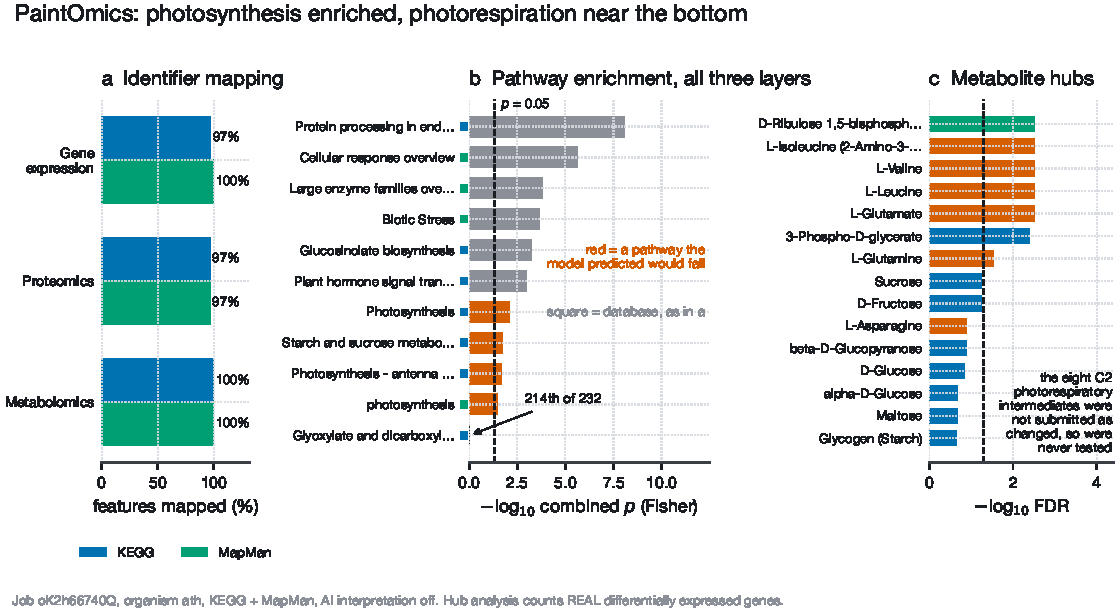
\includegraphics[width=\textwidth]{fig06_paintomics.pdf}
\caption{\textbf{PaintOmics 4 multi-omics pathway integration and empirical metabolite hub neighbourhood test.}
\textbf{a}, Feature coverage across KEGG and MapMan databases.
\textbf{b}, Combined pathway enrichment ranking across 232 pathways (\texttt{T08\_paintomics\_significant.tsv}, \texttt{T09\_paintomics\_carbon.tsv}): endoplasmic reticulum protein processing (UPR, $p = 8.6\times 10^{-9}$) dominates globally; Photosynthesis ($p = 0.008$) and Antenna proteins ($p = 0.022$) reach uncorrected significance, while Glyoxylate and dicarboxylate metabolism (photorespiration) ranks 214th of 232 ($p = 0.994$, bottom $8\%$).
\textbf{c}, Empirical metabolite hub analysis (\texttt{T10\_metabolite\_hubs.tsv}), testing each compound's immediate KEGG reaction neighbourhood for enrichment of measured OSD-522 DEGs: 7 of 15 hubs reach $\mathrm{FDR}<0.05$, exclusively in carbohydrate supply and amino-acid starvation blocks (\texttt{fig06\_paintomics.pdf}).}
\label{fig:paintomics}
\end{figure*}

%-----------------------------------------------------------------------------
\subsection{Cross-study evaluation across five OSDR spaceflight experiments: illumination separates all six flight contrasts}\label{sec:ladder}

Finally, we tested whether the carbon-starvation and photorespiratory signatures scale across the ISS hardware ladder by assembling all available NASA OSDR \textit{Arabidopsis} spaceflight studies that met strict pre-specified inclusion criteria: (i) green shoot, leaf, or whole-seedling tissue (excluding root-only studies because leaf photosynthetic gas transport makes no prediction for roots); (ii) RNA-seq with deposited GeneLab differential expression tables; and (iii) flight-versus-ground contrasts matched on genotype, ecotype, and illumination (\texttt{data/study\_registry.tsv}; Table~\ref{tab:studies}). Five studies yielding six matched contrasts met these criteria: sealed lit \textbf{OSD-522} (BRIC-LED, $60\,\ums$), sealed dark \textbf{OSD-38} (BRIC-20) and \textbf{OSD-321} (BRIC-22), micropore-taped \textbf{OSD-678} (CARA, matched Col-0 lit cabin-wall and dark arms), and actively ventilated lit \textbf{OSD-427} (APEX-04 / VEGGIE, $120\,\ums$) \citep{osd522,osd38,osd321,osd678,osd427}.

\begin{table*}[tbp]
\caption{\textbf{NASA OSDR spaceflight studies evaluated in the cross-study hardware and illumination ladder.}
Audit registry (\texttt{data/study\_registry.tsv}) listing the five included studies (six matched flight-versus-ground contrasts) and six excluded studies with hardware class, tissue, genotype, mission duration, illumination, and inclusion/exclusion rationale.}
\label{tab:studies}
\centering
\footnotesize
\resizebox{\textwidth}{!}{%
\begin{tabular}{llllllll}
\toprule
\textbf{Study} & \textbf{Hardware} & \textbf{Seal class} & \textbf{Tissue} & \textbf{Genotype} & \textbf{Duration} & \textbf{Light regime} & \textbf{Status / Reason} \\
\midrule
OSD-522 & BRIC-LED & Sealed & Shoots & Col-0 WT & $11\,\mathrm{d}$ & Lit ($60\,\ums$) & Included \\
OSD-38 & BRIC-PDFU & Sealed & Seedlings & Col-0 WT & $8\,\mathrm{d}$ & Dark & Included \\
OSD-321 & BRIC-PDFU & Sealed & Seedlings & Col-0 WT & $14\,\mathrm{d}$ & Dark & Included \\
OSD-678 (lit) & CARA plate & Micropore tape & Leaves & Col-0 WT & $12\,\mathrm{d}$ & Lit ($4\text{--}6\,\ums$) & Included \\
OSD-678 (dark) & CARA plate & Micropore tape & Leaves & Col-0 WT & $12\,\mathrm{d}$ & Dark & Included \\
OSD-427 & VEGGIE (VPS) & Ventilated & Leaves & Col-0 WT & $21\,\mathrm{d}$ & Lit ($120\,\ums$) & Included \\
\midrule
OSD-120 & CARA plate & Micropore tape & Root tips & Col-0, Wass. & $12\,\mathrm{d}$ & Lit / Dark & Excluded (roots only) \\
OSD-193 & APH / APEX & Ventilated & Roots & Col-0, \textit{sku6} & $14\,\mathrm{d}$ & Lit & Excluded (roots only) \\
OSD-281 & APH / APEX & Ventilated & Roots & WS, \textit{sku5} & $14\,\mathrm{d}$ & Lit & Excluded (roots only) \\
OSD-218 & APH / APEX & Ventilated & Unstated & Col-0, WS & $14\,\mathrm{d}$ & Lit & Excluded (tissue unstated) \\
OSD-16 & APEX-TAGES & Ventilated & Leaf / stem & Col-0 WT & $12\,\mathrm{d}$ & Lit & Excluded (no DGE table) \\
OSD-7 & ABRS / TAGES & Ventilated & Whole plant & Col-0 WT & $12\,\mathrm{d}$ & Lit & Excluded (microarray) \\
\bottomrule
\end{tabular}%
}
\end{table*}

\begin{figure*}[tbp]
\centering
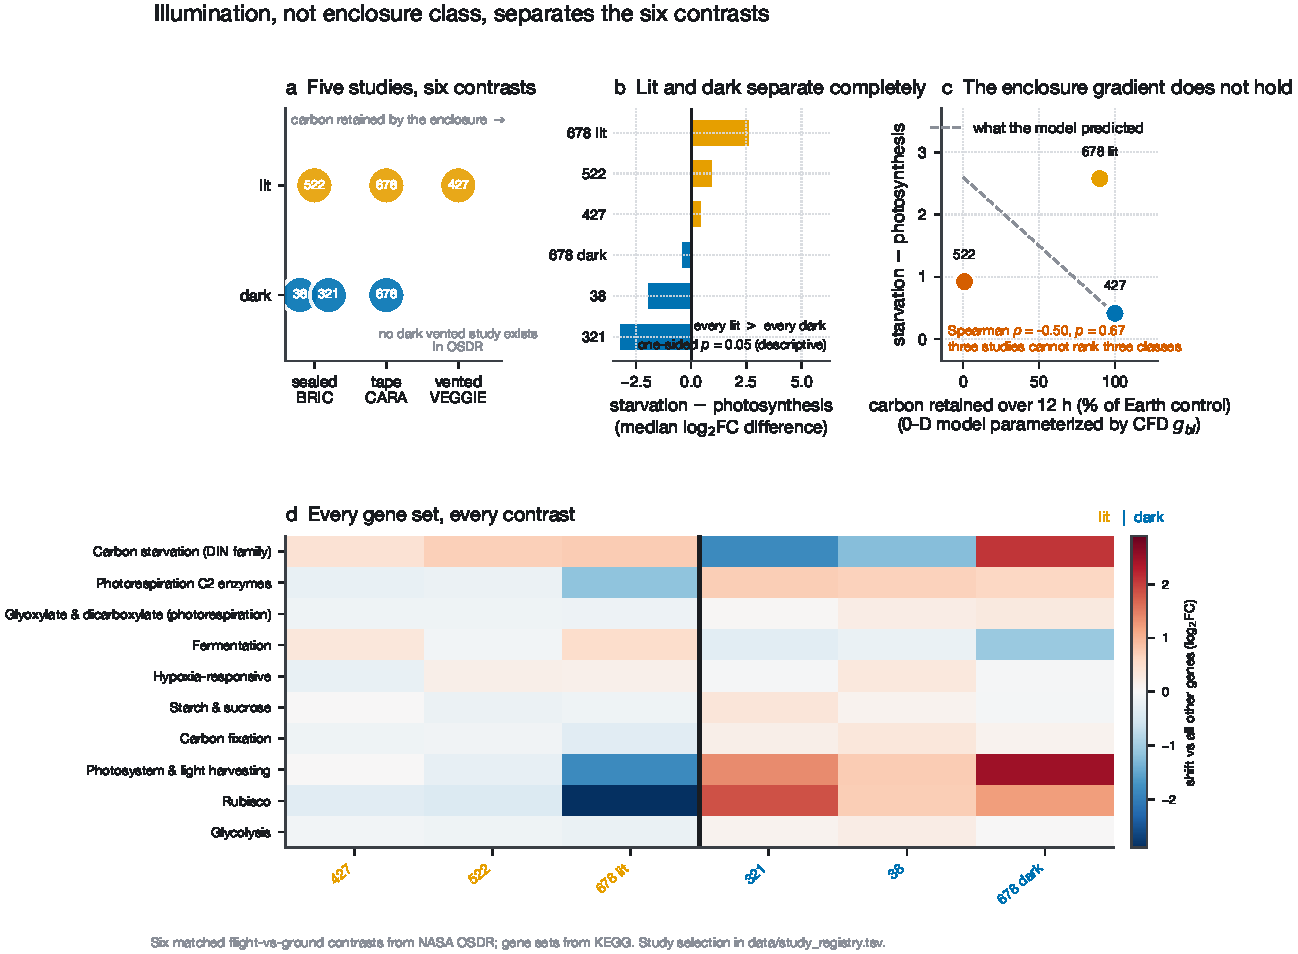
\includegraphics[width=0.52\textwidth]{fig07_hardware_ladder.pdf}\hfill
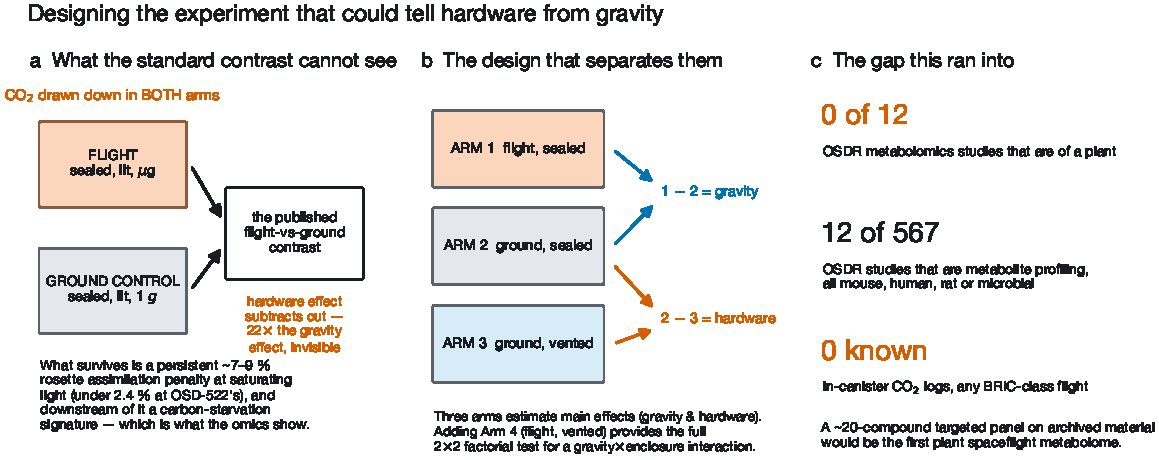
\includegraphics[width=0.46\textwidth]{fig08_implications.pdf}
\caption{\textbf{Cross-study evaluation across six OSDR flight contrasts and experimental design to unconfound hardware from microgravity.}
\textbf{Left} (\texttt{fig07\_hardware\_ladder.pdf}): \textbf{a}, Matrix of six flight-versus-ground contrasts across five OSDR studies. \textbf{b}, Illumination separates all three lit contrasts ($+0.41$, $+0.92$, $+2.58$) from all three dark contrasts ($-0.39$, $-1.95$, $-3.22$; one-sided Mann--Whitney $p = 0.05$) on the carbon-starvation (\textit{DIN}) over photosynthesis contrast (\texttt{T12\_ladder\_contrasts.tsv}). \textbf{c}, Among lit studies, the predicted monotonic gradient across enclosure classes does not hold ($\rho = -0.50$, $p = 0.67$), with dimly lit CARA (\texttt{OSD-678}, $4\text{--}6\,\ums$) sitting highest. \textbf{d}, Heatmap of Mann--Whitney shifts across all ten evaluated gene sets (\texttt{T11\_hardware\_ladder.tsv}).
\textbf{Right} (\texttt{fig08\_implications.pdf}): \textbf{a}, Why standard two-arm spaceflight designs (sealed flight vs.\ sealed ground) cancel the $22\times$ hardware starvation effect while measuring microgravity in carbon-starved plants. \textbf{b}, Proposed three-arm (adding vented ground) and $2\times 2$ factorial (adding vented flight) designs that separate main effects of enclosure atmosphere, microgravity, and their interaction. \textbf{c}, Summary of the OSDR plant metabolomics and in-canister logging archive gaps.}
\label{fig:ladder_implications}
\end{figure*}

Evaluating the ten gene sets and set-versus-set contrasts across all six studies (\texttt{T11\_hardware\_ladder.tsv}, \texttt{T12\_ladder\_contrasts.tsv}; Fig.~\ref{fig:ladder_implications} left) revealed two sharp empirical findings:
\begin{enumerate}
    \item \textbf{Illumination completely separates the six spaceflight contrasts}: On the primary carbon-starvation-over-photosynthesis contrast ($\text{\textit{DIN}} - \text{photosynthesis apparatus}$), \textbf{every illuminated contrast is positive} ($+0.41$ in VEGGIE OSD-427, $+0.92$ in BRIC-LED OSD-522, and $+2.58$ in lit CARA OSD-678) and \textbf{every dark contrast is negative} ($-0.39$ in dark BRIC OSD-38, $-1.95$ in dark BRIC OSD-321, and $-3.22$ in dark CARA OSD-678; descriptive one-sided Mann--Whitney $p = 0.05$; Fig.~\ref{fig:ladder_implications}b). This separation is physically consistent with our central mechanism: photosynthetic $\mathrm{CO_2}$ drawdown and boundary-layer $\mathrm{CO_2}$ depletion require light; in darkness, respiration releases $\mathrm{CO_2}$ rather than consuming it.
    \item \textbf{The simple one-dimensional ranking across enclosure classes does not hold}: Among the three illuminated contrasts, sealed BRIC-LED ($+0.92$) sits above ventilated VEGGIE ($+0.41$) as predicted, but the dimly lit CARA plates in OSD-678 ($+2.58$, grown in only $4\text{--}6\,\ums$ of ambient cabin light near the light compensation point, and with unrecorded plate-sealing tape geometry in OSDR) sit highest (Spearman $\rho = -0.50$, $p = 0.67$; Fig.~\ref{fig:ladder_implications}c).
\end{enumerate}

%=============================================================================
\section{Discussion}\label{sec:discussion}
%=============================================================================

\subsection{Two distinct physical scales of gas transport in spaceflight plant biology}

By uniting a validated 2-D lattice-Boltzmann fluid and mass-transport solver with a mechanistic FvCB Rubisco model and testing their combined predictions across NASA OSDR, this study resolves a longstanding ambiguity in spaceflight plant biology. Two distinct transport bottlenecks operate simultaneously in orbital plant experiments, but at different spatial scales and with different consequences for differential multi-omics:
\begin{enumerate}
    \item \textbf{The microgravity boundary layer ($\sim 0.7\text{--}11\,\mathrm{mm}$, $C_a \to C_s$)} is a genuine gravity effect. Eliminating buoyancy-driven convection reduces $g_{bl}$ by $2.0\text{--}2.3\times$ across single leaves, rosettes, and canopies (Table~\ref{tab:cfd_sweep}). At ambient $\mathrm{CO_2}$ ($400\,\mathrm{ppm}$) and moderate-to-high irradiance, this boundary-layer thickening depresses chloroplastic $C_c$, elevates Rubisco oxygenation $\varphi$, and reduces net assimilation by $5\text{--}9\%$ in leaves/rosettes and $26\text{--}29\%$ in dense microgreen canopies (or $<3\%$ and $11\%$ at $60\,\ums$; Fig.~\ref{fig:fvcb}c). Because this penalty is purely diffusive, horizontal forced ventilation of $\approx 2.0\,\cmsu$ (single leaf) to $\approx 6.1\,\cmsu$ (rosette) completely restores Earth-equivalent boundary-layer conductance (Fig.~\ref{fig:fan_scale}).
    \item \textbf{Enclosure headspace drawdown ($10^1\text{--}10^2\,\mathrm{mm}$, $C_{\text{cabin}} \to C_a$)} is a hardware effect. In an illuminated, hermetically sealed canister such as BRIC-LED, photosynthetic uptake exhausts the $\sim 400\,\mathrm{ppm}$ headspace $\mathrm{CO_2}$ to the compensation point in $\sim 7\,\mathrm{min}$, slashing 12\,h carbon gain to $\approx 1\%$ of an unenclosed control and driving Rubisco oxygenation $\varphi$ from $18\%$ to $46\%$ (Fig.~\ref{fig:hardware}, Fig.~\ref{fig:fvcb}). This enclosure effect is $\approx 22\times$ larger than the microgravity boundary-layer effect, and because it is a volume mass balance, it occurs in the $1\,g$ ground control canister just as rapidly as in flight.
\end{enumerate}

This interaction explains why the microgravity boundary-layer penalty and canister carbon starvation cannot be treated as simple additive stresses. As canister $\mathrm{CO_2}$ falls toward the compensation point, net assimilation $A$ approaches zero, so the concentration drop across the boundary layer ($\Delta C_{bl} = A/g_{bl}$) vanishes and the $1\,g$ and $\mu g$ operating points converge (Fig.~\ref{fig:fvcb}b). Likewise, inside a sealed BRIC Petri dish, transpirational humidification saturates the shallow $7.4\,\mathrm{mm}$ headspace within $1\text{--}2\,\mathrm{min}$, extinguishing solutal buoyancy at $1\,g$ so that even the physical conductances $g_{bl}(1\,g)$ and $g_{bl}(0\,g)$ converge (Supplementary Fig.~\ref{fig:s_dish_feedback}). Consequently, a flight-versus-ground comparison in illuminated sealed hardware measures the residual effect of microgravity inside plants that their own growth canister has already severely carbon-starved (Fig.~\ref{fig:ladder_implications} right). Consistent with this transport-limited framework, whole-stand gas exchange of wheat in microgravity is indistinguishable from $1\,g$ at saturating $\mathrm{CO_2}$ \citep{monje2005}---the exact regime in which boundary-layer and enclosure $\mathrm{CO_2}$ limitations are relieved.

\subsection{What the model explains in the spaceflight multi-ome, and what it does not}

In OSD-522 (BRIC-LED), the coupled model accurately predicted eight of nine directional gene-set shifts in the transcriptome and four of seven in the proteome, including concerted repression of photosystems, Rubisco, Calvin-cycle enzymes, and starch/sucrose synthesis, strong induction of \textit{DIN6/ASN1} carbon-starvation markers, and selective preservation of photorespiratory enzymes relative to Rubisco ($+0.239\,\log_2\mathrm{FC}$ in RNA-seq, $+0.285$ in proteomics; Table~\ref{tab:falsification}). Across five independent OSDR experiments (six matched contrasts), illumination completely separated all lit contrasts from all dark contrasts on the starvation-over-photosynthesis axis (Fig.~\ref{fig:ladder_implications}b).

Equally important are the three places where the data falsified or exceeded the gas-transport model:
\begin{enumerate}
    \item \textbf{Dominance of the endoplasmic reticulum unfolded protein response (UPR)}: The single strongest pathway enrichment in OSD-522 is ER protein processing (\texttt{ath04141}, $p = 8.6\times 10^{-9}$; Fig.~\ref{fig:paintomics}b), a conserved spaceflight stress signature also highlighted in OSD-321 \citep{osd321} that leaf gas transport does not explain. Biophysical and metabolic models of spaceflight adaptation must therefore treat ER proteostasis alongside gas transport rather than assuming a single master stressor.
    \item \textbf{Absence of global photorespiratory pathway enrichment}: Although photorespiratory enzymes were maintained relative to repressed Rubisco, \texttt{ath00630} (glyoxylate and dicarboxylate metabolism) ranked 214th of 232 pathways in PaintOmics ($p = 0.994$), confirming that sealed-canister drawdown cancels between flight and ground arms rather than producing a large net flight-versus-ground photorespiratory induction.
    \item \textbf{Irradiance and sealing confounders across the cross-study ladder}: Among illuminated studies, OSD-678 (CARA) showed the largest starvation-over-photosynthesis shift despite using micropore tape, likely because its lit arm grew in only $4\text{--}6\,\ums$ of cabin light (near the photosynthetic light compensation point) and because exact tape area/permeance is not standardized in OSDR metadata.
\end{enumerate}

\subsection{Limitations and roadmap for spaceflight hardware and experimental design}

Several limitations bound our conclusions. First, the lattice-Boltzmann solver is two-dimensional and employs the Boussinesq approximation ($\beta\Delta C \lesssim 0.5$) and low-Mach limit ($\mathrm{Ma}\le 0.3$). While $1\,g$ convective conductances are insensitive to chamber domain size ($\le 7\%$ change when domain dimensions are doubled; Supplementary Fig.~\ref{fig:s_domain_size} and Table~\ref{tab:s_domain}), $0\,g$ pure-diffusion conductances in 2-D depend logarithmically on the distance to the ambient boundary ($g_{bl}$ dropping $33\%$ for a leaf and $41\%$ for a rosette when the box is doubled), making our open-box $1\,g/\mu g$ ratios conservative lower bounds and motivating full 3-D WebGPU simulations for dense canopies requiring turbulent through-flow. Second, wet-agar boundary conditions (\texttt{agarH2O = 1.3}) are numerically valid at $0\,g$ ($g_{bl} = 0.185\text{--}0.192\,\molms$), but exceed the small-perturbation Boussinesq limit at $1\,g$ ($\beta\Delta C\approx 1.3$) under both BGK and MRT collision schemes (\texttt{T23}, \texttt{T24}; Supplementary Table~\ref{tab:s_real_dish}). Third, stomatal conductance ($g_s = 0.20\,\molms$) and mesophyll conductance ($g_m = 0.30\,\molms$) were held fixed at literature values rather than dynamically coupled to guard-cell $\mathrm{CO_2}$/humidity signalling.

Three concrete experimental actions will resolve the hardware-versus-microgravity confound in future missions (Fig.~\ref{fig:ladder_implications} right):
\begin{enumerate}
    \item \textbf{In-canister $\mathrm{CO_2}$, $\mathrm{O_2}$, and relative humidity logging}: Embedding miniature nondispersive infrared (NDIR) $\mathrm{CO_2}$ and optical $\mathrm{O_2}$ sensors inside BRIC and CARA hardware will convert our 0-D drawdown model into a direct measurement and render the archival BRIC transcriptome record quantitatively re-interpretable.
    \item \textbf{A targeted 20-compound spaceflight plant metabolomics panel}: Profiling the 21 compounds in Table~\ref{tab:s_metabolite_mapping} (phosphoglycolate, glycolate, glycine, serine, 3-PGA, RuBP, sucrose, hexoses, maltose, Asn, BCAAs, Gln, Glu) on archived flight tissues will fill the complete absence of plant metabolomes in NASA OSDR (\texttt{T03}).
    \item \textbf{Three-arm or $2\times 2$ factorial ground controls}: Adding a ventilated ground control arm (or flying paired sealed and ventilated hardware in a $2\times 2$ Gravity $\times$ Enclosure factorial design; Fig.~\ref{fig:ladder_implications}b right) separates the $22\times$ enclosure starvation main effect from the true microgravity main effect and their interaction.
\end{enumerate}

%=============================================================================
\section{Materials and Methods}\label{sec:methods}
%=============================================================================

\subsection{Two-dimensional lattice-Boltzmann fluid and multi-species transport solver}

Incompressible fluid flow was solved on a uniform two-dimensional Cartesian lattice ($\Delta x = 0.288\,\mathrm{mm}$, $\Delta t = 0.173\,\mathrm{ms}$) using the D2Q9 Bhatnagar--Gross--Krook (BGK) lattice-Boltzmann equation (\texttt{src/solver/lbm/LBMFluid.ts}):
\begin{equation}
f_i(\mathbf{x}+\mathbf{c}_i\Delta t, t+\Delta t) - f_i(\mathbf{x},t) = -\frac{1}{\tau_f}\left[f_i(\mathbf{x},t) - f_i^{\mathrm{eq}}(\rho,\mathbf{u})\right] + \Delta t\,F_i(\mathbf{x},t),
\label{eq:lbm_bgk}
\end{equation}
where $\mathbf{c}_i$ ($i=0,\dots,8$) are the discrete D2Q9 velocity vectors, $c_s = 1/\sqrt{3}$ is the lattice speed of sound, $\nu = c_s^2(\tau_f - \tfrac{1}{2}) = 0.02$ is the kinematic viscosity in lattice units, and $F_i$ is the discrete body-force term implemented via the exact second-order Guo forcing scheme \citep{guo2002}. An opt-in multiple-relaxation-time (MRT) collision operator in moment space \citep{lallemand2000} (\texttt{collision: 'mrt'}) was also implemented and verified across all four benchmark gates (\texttt{validation/mrt\_check.ts}). Solid leaf and chamber wall nodes enforce no-slip velocity boundary conditions via halfway bounce-back.

Three gas species ($k \in \{\mathrm{CO_2}, \mathrm{O_2}, \mathrm{H_2O}\}$, stored as concentration excess over cabin ambient $c_k = C_k - C_{k,0}$) were transported simultaneously on D2Q5 advection--diffusion lattices (\texttt{src/solver/lbm/ScalarField.ts}) sharing the macroscopic fluid velocity $\mathbf{u}$:
\begin{multline}
g_{k,j}(\mathbf{x}+\mathbf{e}_j\Delta t, t+\Delta t) - g_{k,j}(\mathbf{x},t) = \\
-\frac{1}{\tau_k}\left[g_{k,j}(\mathbf{x},t) - g_{k,j}^{\mathrm{eq}}(c_k,\mathbf{u})\right] + \Delta t\,w_j S_k(\mathbf{x},t),
\label{eq:lbm_d2q5}
\end{multline}
with lattice diffusivities $D_k = c_{s,5}^2(\tau_k - \tfrac{1}{2})$ set to $0.033 : 0.042 : 0.050$ matching the physical molecular diffusivity ratio $D_{\mathrm{CO_2}} : D_{\mathrm{O_2}} : D_{\mathrm{H_2O}} = 1.6 : 2.0 : 2.4 \times 10^{-5}\,\mseu$ at $25\,^\circ\mathrm{C}$. Gravity couples to the flow via a solutal Boussinesq body force (\texttt{src/solver/lbm/buoyancy.ts}):
\begin{equation}
\mathbf{f}(\mathbf{x},t) = \rho\,\mathbf{g}\sum_k \beta_k\left(c_k(\mathbf{x},t) - c_{k,\mathrm{ref}}\right),
\label{eq:boussinesq}
\end{equation}
where $\mathbf{g} = (0, -g)$ is scaled from $1\,g$ ($9.81\,\msq$) through Mars ($0.378\,g$), Moon ($0.165\,g$), and microgravity ($0\,g$), and $c_{k,\mathrm{ref}}$ is either cabin ambient ($0$, for open/vented scenes) or the instantaneous enclosure mean (\texttt{buoyancyRef: 'enclosureMean'}, preventing uniform background drift in sealed dishes from generating spurious body forces).

\subsection{Plant geometries, spaceflight hardware boundary conditions, and closed-loop feedback}

Three biological architectures were constructed on a $128\times 96$ production lattice ($36.9\times 27.6\,\mathrm{mm}$; refined up to $384\times 288$ in \texttt{validation/resolution\_ladder.ts} and expanded up to $256\times 192$ in \texttt{validation/domain\_size.ts}): (i) an isolated horizontal leaf blade ($52\times 8$ cells, $1.5\,\mathrm{cm}$ chord, plus anatomical outlines and curled transverse sections in \texttt{src/leaf/}); (ii) an overlapping eight-blade rosette (\texttt{rosetteGeometry}, characteristic length $70$ cells); and (iii) a microgreen canopy of nine upright shoots above an adiabatic soil floor (\texttt{canopyGeometry}, $0.3\times$ per-leaf flux for self-shading). Fluid nodes adjacent to leaf solid cells receive stomatal source/sink fluxes ($S_{\mathrm{CO_2}} < 0$, $S_{\mathrm{O_2}} > 0$, $S_{\mathrm{H_2O}} > 0$; reversed and scaled by $R/A = 0.31$ in the dark). Boundary-layer conductance $g_{bl}$ ($\molms$), film thickness $\delta = D_{\mathrm{CO_2}}/g_{bl}$ ($\mathrm{mm}$), and Sherwood number $\mathrm{Sh} = L_{\text{char}}/\delta$ are derived directly from the simulated surface flux and mean surface-to-bulk concentration gap, anchored to $g_{bl}(1\,g,\text{leaf}) = 1.0\,\molms$ (\texttt{T13\_boundary\_layer.csv}).

Hardware boundary conditions on the domain border represent: (i) open reference (anti-bounce-back Dirichlet $c_k = 0$); (ii) sealed BRIC (zero-flux bounce-back, \texttt{membraneK = 0}); (iii) micropore-taped CARA (semi-permeable relaxation $c_k \leftarrow (1 - k_{\mathrm{mem}})c_k$ on perimeter fluid cells each step, \texttt{membraneK = 0.01}); and (iv) ventilated VEGGIE (horizontal channel with density-matched equilibrium inlet at fan speed $U$ and pressure-pinned outlet $\rho = 1$). When closed-loop $\mathrm{CO_2}$ feedback is enabled (\texttt{co2Ambient = 8}), local surface uptake scales as $m_{\mathrm{CO_2}}(c) = [(C_a + c - \Gamma)/(C_a + c - \Gamma + K_C)] / m_{\mathrm{amb}}$ with $\Gamma = 0.125\,C_a$ and $K_C = 0.75\,C_a$. When humidity-limited transpiration is enabled (\texttt{h2oSatExcess = 1.3}), local $\mathrm{H_2O}$ release scales as $\max(0, 1 - c_{\mathrm{H_2O}}/c_{\mathrm{sat}})$.

\subsection{Coupled 0-D enclosure mass balance and Farquhar--von Caemmerer--Berry (FvCB) model}

Canister-scale $\mathrm{CO_2}$ drawdown over a $12\,\mathrm{h}$ photoperiod (\texttt{validation/feedback\_0d.py}, \texttt{scripts/enclosure\_sensitivity.py}) integrates the ordinary differential equation for well-mixed headspace concentration $C_a(t)$ in volume $V = 30\,\mathrm{mL}$ over leaf area $A_{\text{leaf}} = 3\,\mathrm{cm^2}$ and dish seal area $A_{\text{dish}} = 28\,\mathrm{cm^2}$:
\begin{equation}
\rho_{\mathrm{air}}V\frac{\mathrm{d}C_a}{\mathrm{d}t} = -A_{\text{leaf}}\,A_{\mathrm{net}}(C_s(t)) + A_{\text{dish}}\,k_{\mathrm{seal}}\left(C_{\mathrm{cabin}} - C_a(t)\right),
\label{eq:0d_mass_balance}
\end{equation}
where $\rho_{\mathrm{air}} = 41.6\,\mathrm{mol\,m^{-3}}$ ($25\,^\circ\mathrm{C}$), $k_{\mathrm{seal}} = 0$ (BRIC), $0.006\,\molms$ (CARA micropore tape), or $\infty$ (VEGGIE), and $C_s(t)$ is coupled to $C_a(t)$ through $g_{bl}$.

In \texttt{scripts/fvcb.py} (mirrored to $10^{-6}$ parity in \texttt{public/explorer/app/fvcb.js}), steady-state $g_{bl}$ from \texttt{T13\_boundary\_layer.csv} is placed in series with stomatal conductance $g_s = 0.20\,\molms$ and mesophyll conductance $g_m = 0.30\,\molms$ to give total conductance to Rubisco:
\begin{equation}
g_{\mathrm{tot}} = \left(\frac{1}{g_{bl}} + \frac{1}{g_s} + \frac{1}{g_m}\right)^{-1}, \qquad C_c = C_a - \frac{A}{g_{\mathrm{tot}}}.
\label{eq:gtot}
\end{equation}
Biochemical demand $A(C_c) = \min(A_c, A_j) - R_d$ is solved simultaneously with diffusive supply (Eq.~\ref{eq:gtot}) by bisection over $C_c \in [\Gamma^*, C_a]$ using Bernacchi et al.~\citep{bernacchi2001,bernacchi2003} temperature responses at $25\,^\circ\mathrm{C}$ ($V_{c\max,25} = 90.0\,\ums$, $J_{\max,25} = 153.0\,\ums$, $R_{d,25} = 1.35\,\ums$, $K_{c,25} = 404.9\,\mu\mathrm{mol\,mol^{-1}}$, $K_{o,25} = 278.4\,\mathrm{mmol\,mol^{-1}}$, $\Gamma^*_{25} = 42.75\,\mu\mathrm{mol\,mol^{-1}}$ at $O_{\mathrm{ref}} = 210\,\mathrm{mmol\,mol^{-1}}$; Supplementary Table~\ref{tab:s_fvcb_params}). Local surface $\mathrm{O_2}$ build-up from CFD shifts the compensation point as $\Gamma^*(T, O_{\mathrm{local}}) = \Gamma^*(T)\cdot(O_{\mathrm{local}}/O_{\mathrm{ref}})$. From the fixed-point solution $(C_c, A)$, carboxylation rate $V_c = (A + R_d)/(1 - \Gamma^*/C_c)$, oxygenation rate $V_o = 2(\Gamma^*/C_c)V_c$, photorespiration $R_p = 0.5\,V_o$, and oxygenation fraction $\varphi = V_o/(V_o+V_c)$ are evaluated exactly.

\subsection{NASA OSDR multi-omics processing, gene-set falsification, and PaintOmics 4 integration}

Unnormalized RSEM gene-level counts for OSD-522 ($n=6$ flight, $n=6$ ground shoot libraries) were retrieved via the NASA OSDR API (\texttt{scripts/00\_fetch\_osdr.py}) and analyzed with PyDESeq2 \citep{pydeseq2} (\texttt{scripts/01\_dge\_rnaseq.py}) using design $\sim\texttt{condition}$ with Cook's distance outlier refitting and independent filtering (\texttt{T01\_osd522\_transcriptome.tsv}). Deposited TMT soluble and membrane shoot proteomics tables from OSD-522 were merged by UniProt/AGI accession (\texttt{scripts/02\_prep\_proteomics.py}, \texttt{T02\_osd522\_proteome.tsv}). Gene sets (\texttt{scripts/genesets.py}) were retrieved live from the KEGG REST API \citep{kanehisa2000,kegg} (\texttt{ath00630}, \texttt{ath00710}, \texttt{ath00500}, \texttt{ath00010}, \texttt{ath00195}, \texttt{ath00196}) alongside curated Araport11 locus sets for core photorespiratory enzymes (\texttt{photorespiration\_core}, $n=13$), Rubisco ($n=5$), \textit{DIN} carbon-starvation markers ($n=5$), fermentation ($n=6$), and core hypoxia markers ($n=3$). Directional falsification tests (\texttt{scripts/04\_falsification\_check.py}) used two-sided Mann--Whitney $U$ tests of gene-set $\log_2\mathrm{FC}$ distributions against the genome-wide background (\texttt{T07\_falsification\_osd522.tsv}). Multi-omics pathway enrichment was performed in PaintOmics 4 \citep{paintomics4} across KEGG and MapMan ontologies (saved job record \texttt{oK2h66740Q}, verified against metabolite-free control \texttt{T17\_integration\_control\_nometa.tsv} and external Fisher/Mann--Whitney tests \texttt{T16\_independent\_pathways.tsv}). MapMan pathway membership (\texttt{scripts/mapman.py}) was reconstructed deterministically from GoMapMan Araport11 bin assignments and vendored MapManStore diagram layouts (\texttt{data/mapman/PROVENANCE.md}). Cross-study evaluation (\texttt{scripts/07\_hardware\_ladder.py}) ingested GeneLab differential expression tables for OSD-522, OSD-38, OSD-321, OSD-678, and OSD-427 according to the audit rules in \texttt{data/study\_registry.tsv}.

\subsection{Use of AI coding and drafting assistants}

In accordance with publisher guidelines on artificial intelligence transparency, the author discloses that AI coding and drafting assistants (Claude Code, Anthropic; Google Antigravity) were used under the author's direct supervision to implement solver and pipeline scripts, generate figures, and format manuscript drafts. The author independently verified all physical equations, numerical validation gates, OSDR data processing, statistical tests, and bibliographic citations, and takes full responsibility for the integrity of the work.

%=============================================================================
\section*{Data and Code Availability}
%=============================================================================

All source code (TypeScript/React 2-D lattice-Boltzmann CFD workbench, headless validation suite, Python FvCB and multi-omics pipeline, and interactive web applications), derived tables (\texttt{T1}--\texttt{T24} and \texttt{T01}--\texttt{T17} with machine-verified provenance in \texttt{results/MANIFEST.tsv}), publication figures, and LaTeX/Word manuscript sources are openly available at \url{https://github.com/dr-richard-barker/Spaceflight-Plant-Biophysics-Multiomics} under the MIT (code) and CC-BY-4.0 (manuscript and figures) licenses, and archived on Zenodo. Primary spaceflight multi-omics datasets are publicly available in the NASA Open Science Data Repository \citep{osdr2025} under accessions OSD-522 \citep{osd522}, OSD-38 \citep{osd38}, OSD-321 \citep{osd321}, OSD-678 \citep{osd678}, and OSD-427 \citep{osd427}. Empirical whole-plant chamber gas-exchange data from Chew et al.~\citep{chew2022} are archived at Edinburgh DataShare (\url{https://doi.org/10.7488/ds/3453}) \citep{chew2022data}.

\section*{CRediT Authorship Contribution Statement}
\textbf{Richard J. Barker}: Conceptualization, Methodology, Software, Validation, Formal analysis, Investigation, Data Curation, Writing -- Original Draft, Writing -- Review \& Editing, Visualization.

\section*{Declaration of Competing Interest}
The author declares that he has no known competing financial interests or personal relationships that could have appeared to influence the work reported in this paper.

\section*{Funding}
This research did not receive any specific grant from funding agencies in the public, commercial, or not-for-profit sectors.

\section*{Acknowledgements}
The author thanks Y.~H. Chew and A.~J. Millar (University of Edinburgh) for open whole-plant chamber gas-exchange datasets, the NASA Open Science Data Repository (OSDR / GeneLab) team and Analysis Working Groups, and the spaceflight plant biology investigators who generated the archival flight datasets analyzed here.

\bibliographystyle{elsarticle-num}
\bibliography{references}

\end{document}
